\documentclass[aspectratio=169, 11pt]{beamer}

\usetheme{Madrid}
\usecolortheme{whale}
\setbeamercolor{frametitle}{bg=blue!8, fg=black}
\setbeamercolor{title}{bg=blue!12, fg=black}
\setbeamercolor{structure}{fg=blue!50!black}
\setbeamercolor{item}{fg=blue!50!black}
\setbeamertemplate{navigation symbols}{}
\setbeamertemplate{footline}{
  \leavevmode\hbox{%
    \begin{beamercolorbox}[wd=.35\paperwidth,ht=2.5ex,dp=1ex,left]{author in head/foot}%
      \hspace*{1em}\footnotesize Machine Learning with R (Dr.\ Endri Ra\c{c}o)
    \end{beamercolorbox}%
    \begin{beamercolorbox}[wd=.35\paperwidth,ht=2.5ex,dp=1ex,center]{title in head/foot}%
      \footnotesize Classification
    \end{beamercolorbox}%
    \begin{beamercolorbox}[wd=.3\paperwidth,ht=2.5ex,dp=1ex,right]{date in head/foot}%
      \footnotesize Week 2, 2025 \hspace*{1em} \insertframenumber{} / \inserttotalframenumber \hspace*{1em}
    \end{beamercolorbox}}%
}

\usepackage{amsmath,amssymb,mathtools}
\usepackage{tikz}
\usetikzlibrary{arrows.meta, positioning, calc, shapes, decorations.pathreplacing, patterns}
\usepackage{pgfplots}
\pgfplotsset{compat=1.18}
\usepackage{booktabs}
\usepackage{xcolor}

\definecolor{accent}{RGB}{59,130,246}
\definecolor{darkblue}{RGB}{30,39,97}
\definecolor{softred}{RGB}{239,68,68}
\definecolor{softgreen}{RGB}{16,185,129}
\definecolor{amber}{RGB}{245,158,11}
\definecolor{muted}{RGB}{100,116,139}
\definecolor{orange}{RGB}{249,115,22}

\title{Classification}
\subtitle{Logistic Regression, LDA, QDA, Naive Bayes \& KNN --- ISLR Chapter 4}
\author{Machine Learning with R}
\institute{Dr.\ Endri Ra\c{c}o}
\date{Week 2, 2025}

\begin{document}

% ═══════════ TITLE ═══════════
\begin{frame}
\titlepage
\end{frame}

% ═══════════ OVERVIEW ═══════════
\begin{frame}{Today's Roadmap}
\begin{columns}
\column{0.5\textwidth}
\begin{enumerate}
  \item Why not linear regression?
  \item Logistic Regression
  \item LDA \& QDA
  \item Naive Bayes
  \item KNN for classification
  \item Confusion matrix \& ROC
  \item Comparing methods
\end{enumerate}

\column{0.45\textwidth}
\textbf{Datasets:}
\begin{itemize}
  \item \texttt{Default} --- credit card default
  \item \texttt{Smarket} --- S\&P 500 direction
  \item \texttt{Weekly} --- weekly returns
  \item \texttt{Boston} --- crime rate
\end{itemize}

\vspace{0.5em}
\textbf{Methods:}

Logistic, LDA, QDA, NB, KNN
\end{columns}
\end{frame}


% ═══════════ THE CLASSIFICATION PROBLEM ═══════════
\begin{frame}{The Classification Problem}
\begin{columns}
\column{0.5\textwidth}
\textbf{Given:}

$(x_1, y_1), \ldots, (x_n, y_n)$

where $y_i \in \{1, 2, \ldots, K\}$

\vspace{0.5em}
\textbf{Goal:}

Build a classifier $C(x)$ that assigns a new observation $x$ to one of $K$ classes

\vspace{0.5em}
\textbf{Often:} First estimate
$$P(Y = k \mid X = x)$$
then classify to the most probable class

\column{0.45\textwidth}
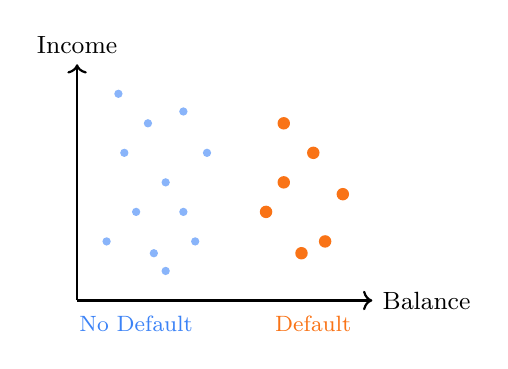
\begin{tikzpicture}[scale=0.75]
  \draw[->, thick] (0,0) -- (5,0) node[right] {\small Balance};
  \draw[->, thick] (0,0) -- (0,4) node[above] {\small Income};
  % No default
  \foreach \x/\y in {0.5/1, 0.8/2.5, 1/1.5, 1.2/3, 1.5/2, 1.3/0.8, 1.8/3.2, 2/1, 0.7/3.5, 1.5/0.5, 2.2/2.5, 1.8/1.5} {
    \fill[accent!60] (\x, \y) circle (2pt);
  }
  % Default
  \foreach \x/\y in {3.2/1.5, 3.5/2, 3.8/0.8, 4/2.5, 4.2/1, 3.5/3, 4.5/1.8} {
    \fill[orange] (\x, \y) circle (3pt);
  }
  \node[accent] at (1, -0.4) {\footnotesize No Default};
  \node[orange] at (4, -0.4) {\footnotesize Default};
\end{tikzpicture}
\end{columns}
\end{frame}


\begin{frame}{A Real Example: Credit Card Default}
\begin{columns}
\column{0.5\textwidth}
\textbf{Default dataset:}

$n = 10{,}000$ customers

\vspace{0.3em}
\begin{tabular}{ll}
\toprule
Variable & Type \\
\midrule
\texttt{default} & Yes/No \\
\texttt{student} & Yes/No \\
\texttt{balance} & \$0--\$2,654 \\
\texttt{income} & \$772--\$73,554 \\
\bottomrule
\end{tabular}

\vspace{0.5em}
Default rate $\approx 3.3\%$

\textcolor{softred}{Imbalanced classes!}

\column{0.45\textwidth}
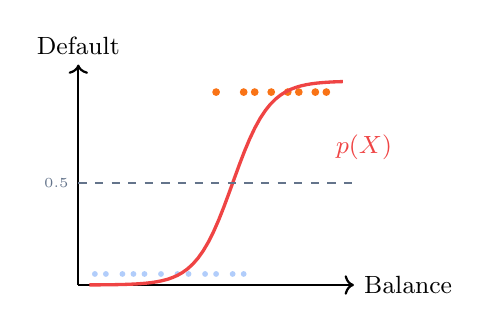
\begin{tikzpicture}[scale=0.7]
  \draw[->, thick] (0,0) -- (5,0) node[right] {\small Balance};
  \draw[->, thick] (0,0) -- (0,4) node[above] {\small Default};
  % 0s
  \foreach \x in {0.3, 0.5, 0.8, 1.0, 1.2, 1.5, 1.8, 2.0, 2.3, 2.5, 2.8, 3.0} {
    \fill[accent!40] (\x, 0.2) circle (1.5pt);
  }
  % 1s
  \foreach \x in {2.5, 3.0, 3.2, 3.5, 3.8, 4.0, 4.3, 4.5} {
    \fill[orange] (\x, 3.5) circle (2pt);
  }
  % Sigmoid
  \draw[softred, very thick, domain=0.2:4.8, samples=50] plot (\x, {3.7/(1+exp(-3*(\x-2.8)))});
  \node[softred, right] at (4.5, 2.5) {\small $p(X)$};
  \draw[muted, dashed] (0, 1.85) -- (5, 1.85);
  \node[muted, left] at (0, 1.85) {\tiny 0.5};
\end{tikzpicture}
\end{columns}
\end{frame}


\begin{frame}{Why Not Linear Regression?}
\begin{columns}
\column{0.48\textwidth}
\textbf{Problem 1: Arbitrary coding}

If $Y \in \{\text{stroke}, \text{OD}, \text{epilepsy}\}$

Code as $Y = 1, 2, 3$?

\vspace{0.2em}
Linear regression implies:\\
OD is ``between'' stroke and epilepsy

\vspace{0.3em}
\textcolor{softred}{Ordering is meaningless!}

\vspace{0.5em}
\textbf{Problem 2: Out-of-range}

$\hat{Y}$ can be $< 0$ or $> 1$

Not a valid probability!

\column{0.48\textwidth}
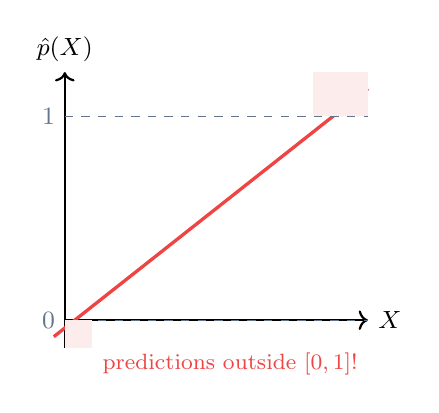
\begin{tikzpicture}[scale=0.7]
  \draw[->, thick] (0,0) -- (5.5,0) node[right] {\small $X$};
  \draw[->, thick] (0,-0.5) -- (0,4.5) node[above] {\small $\hat{p}(X)$};
  % Linear fit going below 0 and above 1
  \draw[softred, very thick] (-0.2, -0.3) -- (5.5, 4.2);
  % Bounds
  \draw[muted, dashed] (0, 3.7) -- (5.5, 3.7);
  \node[muted, left] at (0, 3.7) {\small 1};
  \draw[muted, dashed] (0, 0) -- (5.5, 0);
  \node[muted, left] at (0, 0) {\small 0};
  % Shade bad regions
  \fill[softred!10] (0, -0.5) rectangle (0.5, 0);
  \fill[softred!10] (4.5, 3.7) rectangle (5.5, 4.5);
  \node[softred] at (3, -0.8) {\footnotesize predictions outside $[0,1]$!};
\end{tikzpicture}

\vspace{0.3em}
\textcolor{softgreen}{\textbf{Solution: Logistic regression}}

Outputs are always in $(0, 1)$
\end{columns}
\end{frame}


% ═══════════ LOGISTIC REGRESSION ═══════════
\begin{frame}{Logistic Regression: The Model}

\textbf{Key idea:} Model $P(Y = 1 \mid X)$ directly, ensure it stays in $(0,1)$

$$p(X) = P(Y = 1 \mid X) = \frac{e^{\beta_0 + \beta_1 X}}{1 + e^{\beta_0 + \beta_1 X}}$$

\begin{columns}
\column{0.5\textwidth}
\textbf{The logistic (sigmoid) function:}

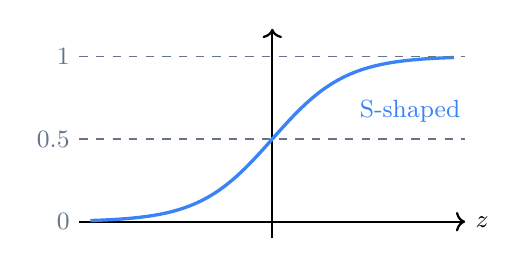
\begin{tikzpicture}[scale=0.7]
  \draw[->, thick] (-3.5,0) -- (3.5,0) node[right] {\small $z$};
  \draw[->, thick] (0,-0.3) -- (0,3.5);
  \draw[accent, very thick, domain=-3.3:3.3, samples=60] plot (\x, {3/(1+exp(-1.5*\x))});
  \draw[muted, dashed] (-3.5, 3) -- (3.5, 3);
  \node[muted, left] at (-3.5, 3) {\small $1$};
  \draw[muted, dashed] (-3.5, 1.5) -- (3.5, 1.5);
  \node[muted, left] at (-3.5, 1.5) {\small $0.5$};
  \node[muted, left] at (-3.5, 0) {\small $0$};
  \node[accent] at (2.5, 2) {\small S-shaped};
\end{tikzpicture}

\column{0.45\textwidth}
\textbf{Properties:}

\begin{itemize}
  \item $p(X) \in (0, 1)$ always
  \item $p(X) = 0.5$ when $\beta_0 + \beta_1 X = 0$
  \item S-shaped curve
  \item Monotonic: as $X \uparrow$, $p$ moves toward 0 or 1
\end{itemize}
\end{columns}
\end{frame}


\begin{frame}{The Odds and the Log-Odds}
\begin{columns}
\column{0.5\textwidth}
\textbf{Odds:}
$$\frac{p(X)}{1 - p(X)} = e^{\beta_0 + \beta_1 X}$$

\begin{tabular}{cc}
\toprule
$p(X)$ & Odds \\
\midrule
0.2 & 1:4 \\
0.5 & 1:1 \\
0.8 & 4:1 \\
0.9 & 9:1 \\
\bottomrule
\end{tabular}

\column{0.45\textwidth}
\textbf{Log-odds (logit):}
$$\log\left(\frac{p(X)}{1 - p(X)}\right) = \beta_0 + \beta_1 X$$

\vspace{0.3em}
The \textbf{logit} is linear in $X$!

\vspace{0.5em}
$\beta_1$: a one-unit increase in $X$ changes the \textbf{log-odds} by $\beta_1$

\vspace{0.3em}
\textit{Not the probability itself ---\\the relationship is non-linear}
\end{columns}
\end{frame}


\begin{frame}{Estimating Coefficients: Maximum Likelihood}
\begin{columns}
\column{0.55\textwidth}
No closed-form solution (unlike OLS)

\vspace{0.3em}
\textbf{Likelihood function:}
$$\ell(\beta_0, \beta_1) = \prod_{i: y_i = 1} p(x_i) \cdot \prod_{i: y_i = 0} (1 - p(x_i))$$

\vspace{0.3em}
Choose $\hat{\beta}_0, \hat{\beta}_1$ to \textbf{maximize} $\ell$

\vspace{0.3em}
Solved numerically (Newton--Raphson)

\vspace{0.3em}
R does it for you: \texttt{glm(..., family = binomial)}

\column{0.4\textwidth}
\textbf{Intuition:}

\vspace{0.3em}
Find coefficients that make the \textbf{observed data most probable}

\vspace{0.5em}
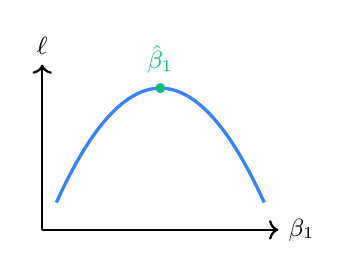
\begin{tikzpicture}[scale=0.6]
  \draw[->, thick] (0,0) -- (5,0) node[right] {\small $\beta_1$};
  \draw[->, thick] (0,0) -- (0,3.5) node[above] {\small $\ell$};
  \draw[accent, very thick, domain=0.3:4.7, samples=50] plot (\x, {-0.5*(\x-2.5)*(\x-2.5) + 3});
  \fill[softgreen] (2.5, 3) circle (3pt);
  \node[softgreen, above] at (2.5, 3.1) {\small $\hat{\beta}_1$};
\end{tikzpicture}
\end{columns}
\end{frame}


\begin{frame}{Worked Example: Default Data}

\begin{columns}
\column{0.5\textwidth}
\texttt{glm(default \textasciitilde{} balance, family = binomial)}

\vspace{0.3em}
\begin{tabular}{lrrl}
\toprule
 & $\hat{\beta}$ & SE & $p$ \\
\midrule
Intercept & $-10.65$ & 0.36 & $<0.001$ \\
balance & $0.0055$ & 0.0002 & $<0.001$ \\
\bottomrule
\end{tabular}

\vspace{0.5em}
\textbf{Interpretation:}

Each \$1 increase in balance $\Rightarrow$\\
log-odds of default increases by $0.0055$

\column{0.45\textwidth}
\textbf{Predict at balance = \$1000:}

$\hat{p} = \dfrac{e^{-10.65 + 0.0055 \times 1000}}{1 + e^{-10.65 + 0.0055 \times 1000}}$

\vspace{0.3em}
$= \dfrac{e^{-5.15}}{1 + e^{-5.15}} = 0.0058$

\vspace{0.3em}
$0.6\%$ chance of default

\vspace{0.5em}
\textbf{At balance = \$2000:}

$\hat{p} = 0.586$ \quad (58.6\%!)
\end{columns}
\end{frame}


\begin{frame}{Multiple Logistic Regression}

$$\log\left(\frac{p(X)}{1 - p(X)}\right) = \beta_0 + \beta_1 X_1 + \beta_2 X_2 + \cdots + \beta_p X_p$$

\begin{columns}
\column{0.5\textwidth}
\textbf{Default: all predictors}

\begin{tabular}{lrr}
\toprule
 & $\hat{\beta}$ & $p$-value \\
\midrule
Intercept & $-10.87$ & $<0.001$ \\
balance & $0.0057$ & $<0.001$ \\
income & $0.0030$ & 0.62 \\
student & $-0.6468$ & $<0.001$ \\
\bottomrule
\end{tabular}

\vspace{0.3em}
\textcolor{softred}{Income is not significant!}

\column{0.45\textwidth}
\textbf{Surprise: Student is negative!}

In simple logistic: student is \textit{positive}

In multiple logistic: student is \textit{negative}

\vspace{0.5em}
\textbf{Why?}

Students have higher \textit{balances}

Controlling for balance, students\\
are \textit{less} likely to default

\vspace{0.3em}
\textcolor{amber}{Confounding --- same as Newspaper!}
\end{columns}
\end{frame}


\begin{frame}{Making Predictions: The Decision Boundary}
\begin{columns}
\column{0.5\textwidth}
\textbf{Default rule:}

Classify to ``Yes'' if $\hat{p}(X) \geq 0.5$

\vspace{0.3em}
Equivalently: classify to ``Yes'' if
$$\hat{\beta}_0 + \hat{\beta}_1 X_1 + \cdots \geq 0$$

\vspace{0.5em}
The \textbf{decision boundary} is the set of $X$ where $\hat{p}(X) = 0.5$

\vspace{0.3em}
For logistic regression: it's a \textbf{linear} boundary

\column{0.45\textwidth}
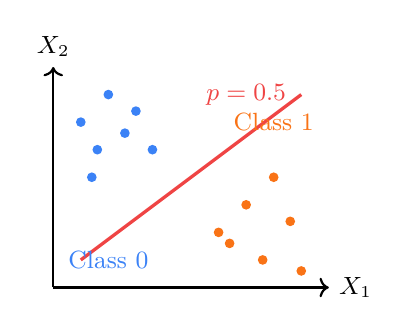
\begin{tikzpicture}[scale=0.7]
  \draw[->, thick] (0,0) -- (5,0) node[right] {\small $X_1$};
  \draw[->, thick] (0,0) -- (0,4) node[above] {\small $X_2$};
  % Two classes
  \foreach \x/\y in {0.5/3, 0.8/2.5, 1/3.5, 1.3/2.8, 1.5/3.2, 0.7/2, 1.8/2.5} {
    \fill[accent] (\x,\y) circle (2.5pt);
  }
  \foreach \x/\y in {3/1, 3.5/1.5, 3.8/0.5, 4/2, 4.3/1.2, 3.2/0.8, 4.5/0.3} {
    \fill[orange] (\x,\y) circle (2.5pt);
  }
  % Decision boundary
  \draw[softred, very thick] (0.5, 0.5) -- (4.5, 3.5);
  \node[softred] at (3.5, 3.5) {\small $p = 0.5$};
  \node[accent] at (1, 0.5) {\small Class 0};
  \node[orange] at (4, 3) {\small Class 1};
\end{tikzpicture}
\end{columns}
\end{frame}


\begin{frame}{Changing the Threshold}

\textbf{What if we use a threshold other than 0.5?}

\vspace{0.3em}
\begin{columns}
\column{0.5\textwidth}
\textbf{Lower threshold} (e.g., 0.2):
\begin{itemize}
  \item More ``Default'' predictions
  \item Catches more true defaults
  \item But more false alarms
\end{itemize}

\vspace{0.3em}
\textbf{Higher threshold} (e.g., 0.8):
\begin{itemize}
  \item Fewer ``Default'' predictions
  \item Misses many true defaults
  \item But very few false alarms
\end{itemize}

\column{0.45\textwidth}
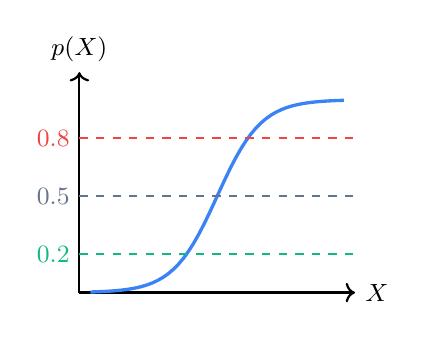
\begin{tikzpicture}[scale=0.7]
  \draw[->, thick] (0,0) -- (5,0) node[right] {\small $X$};
  \draw[->, thick] (0,0) -- (0,4) node[above] {\small $p(X)$};
  \draw[accent, very thick, domain=0.2:4.8, samples=50] plot (\x, {3.5/(1+exp(-2.5*(\x-2.5)))});
  % Threshold lines
  \draw[softgreen, thick, dashed] (0, 0.7) -- (5, 0.7);
  \node[softgreen, left] at (0, 0.7) {\small 0.2};
  \draw[muted, thick, dashed] (0, 1.75) -- (5, 1.75);
  \node[muted, left] at (0, 1.75) {\small 0.5};
  \draw[softred, thick, dashed] (0, 2.8) -- (5, 2.8);
  \node[softred, left] at (0, 2.8) {\small 0.8};
\end{tikzpicture}

\vspace{0.3em}
\centering
\textit{The right threshold depends on the \textbf{cost} of each type of error}
\end{columns}
\end{frame}


% ═══════════ CONFUSION MATRIX ═══════════
\begin{frame}{The Confusion Matrix}

\begin{center}
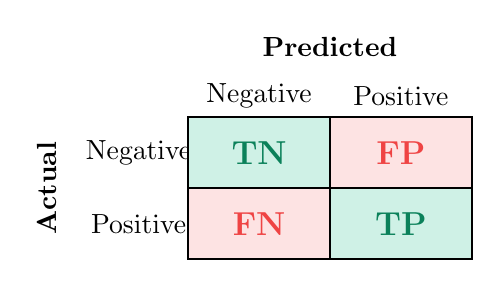
\begin{tikzpicture}[scale=0.9]
  % Headers
  \node[font=\bfseries] at (3.5, 3.5) {Predicted};
  \node[font=\bfseries, rotate=90] at (-0.5, 1.5) {Actual};
  \node at (2.5, 2.8) {Negative};
  \node at (4.5, 2.8) {Positive};
  \node at (0.8, 2) {Negative};
  \node at (0.8, 1) {Positive};

  % Cells
  \fill[softgreen!20] (1.5, 1.5) rectangle (3.5, 2.5);
  \node[font=\large\bfseries, softgreen!70!black] at (2.5, 2) {TN};

  \fill[softred!15] (3.5, 1.5) rectangle (5.5, 2.5);
  \node[font=\large\bfseries, softred] at (4.5, 2) {FP};

  \fill[softred!15] (1.5, 0.5) rectangle (3.5, 1.5);
  \node[font=\large\bfseries, softred] at (2.5, 1) {FN};

  \fill[softgreen!20] (3.5, 0.5) rectangle (5.5, 1.5);
  \node[font=\large\bfseries, softgreen!70!black] at (4.5, 1) {TP};

  % Grid
  \draw[thick] (1.5, 0.5) rectangle (5.5, 2.5);
  \draw[thick] (3.5, 0.5) -- (3.5, 2.5);
  \draw[thick] (1.5, 1.5) -- (5.5, 1.5);
\end{tikzpicture}
\end{center}

\vspace{0.3em}
\begin{columns}
\column{0.48\textwidth}
$\text{Sensitivity} = \dfrac{\text{TP}}{\text{TP} + \text{FN}}$ \quad (true positive rate)

\vspace{0.3em}
$\text{Specificity} = \dfrac{\text{TN}}{\text{TN} + \text{FP}}$ \quad (true negative rate)

\column{0.48\textwidth}
$\text{Precision} = \dfrac{\text{TP}}{\text{TP} + \text{FP}}$

\vspace{0.3em}
$\text{Accuracy} = \dfrac{\text{TP} + \text{TN}}{n}$

\vspace{0.3em}
\textcolor{softred}{\footnotesize Accuracy can be misleading with imbalanced classes!}
\end{columns}
\end{frame}


\begin{frame}{Worked Example: Default Confusion Matrix}

Threshold $= 0.5$, test set $n = 10{,}000$

\begin{columns}
\column{0.45\textwidth}
\begin{center}
\begin{tabular}{lcc}
\toprule
 & Pred.\ No & Pred.\ Yes \\
\midrule
Actual No & 9,627 & 40 \\
Actual Yes & 228 & 105 \\
\bottomrule
\end{tabular}
\end{center}

\vspace{0.3em}
Accuracy $= (9627 + 105)/10000 = 97.3\%$

\textbf{Sounds great?}

\column{0.5\textwidth}
\textbf{But look closer:}

Sensitivity $= 105 / (105 + 228) = 31.5\%$

\textcolor{softred}{We miss 68.5\% of defaulters!}

\vspace{0.5em}
\textbf{Why?}

Only $3.3\%$ default --- predicting ``No'' always gives $96.7\%$ accuracy!

\vspace{0.3em}
$\Rightarrow$ Lower the threshold to catch more defaults
\end{columns}
\end{frame}


\begin{frame}{The ROC Curve}
\begin{columns}
\column{0.5\textwidth}
\textbf{ROC} = Receiver Operating Characteristic

\vspace{0.3em}
Plot \textbf{Sensitivity} vs \textbf{1 $-$ Specificity}\\
for all possible thresholds

\vspace{0.5em}
\textbf{AUC} (Area Under Curve):
\begin{itemize}
  \item AUC $= 0.5$: random guessing
  \item AUC $= 1.0$: perfect classifier
  \item AUC $> 0.8$: good
  \item AUC $> 0.9$: excellent
\end{itemize}

\column{0.45\textwidth}
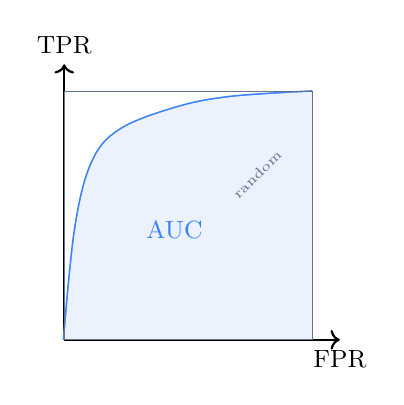
\begin{tikzpicture}[scale=0.7]
  \draw[->, thick] (0,0) -- (5,0) node[below] {\small FPR};
  \draw[->, thick] (0,0) -- (0,5) node[above] {\small TPR};
  % Random
  \draw[muted, dashed] (0,0) -- (4.5,4.5);
  % Good ROC
  \draw[accent, very thick, smooth, tension=0.6] plot coordinates {(0,0)(0.2,2)(0.5,3.2)(1,3.8)(2,4.2)(3,4.4)(4.5,4.5)};
  % Fill AUC
  \fill[accent!10, smooth, tension=0.6] plot coordinates {(0,0)(0.2,2)(0.5,3.2)(1,3.8)(2,4.2)(3,4.4)(4.5,4.5)} -- (4.5,0) -- cycle;
  \node[accent] at (2, 2) {\small AUC};
  \node[muted, rotate=45] at (3.5, 3) {\tiny random};
  \draw[muted] (0,0) rectangle (4.5,4.5);
\end{tikzpicture}
\end{columns}
\end{frame}


% ═══════════ BAYES THEOREM ═══════════
\begin{frame}{Generative Models: A Different Approach}
\begin{columns}
\column{0.55\textwidth}
\textbf{Logistic regression:} models $P(Y \mid X)$ directly

\textbf{Generative approach:} models $P(X \mid Y)$ for each class, then uses Bayes' theorem

\vspace{0.5em}
\textbf{Bayes' Theorem:}
$$P(Y = k \mid X = x) = \frac{\pi_k \cdot f_k(x)}{\sum_{l=1}^{K} \pi_l \cdot f_l(x)}$$

$\pi_k = P(Y = k)$ --- prior probability

$f_k(x) = P(X = x \mid Y = k)$ --- class density

\column{0.4\textwidth}
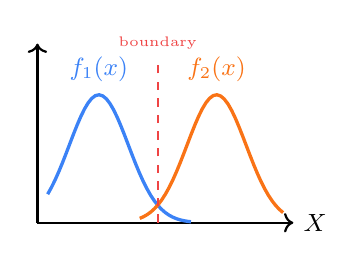
\begin{tikzpicture}[scale=0.65]
  \draw[->, thick] (0,0) -- (5,0) node[right] {\small $X$};
  \draw[->, thick] (0,0) -- (0,3.5);
  % Class 1 density
  \draw[accent, very thick, domain=0.2:3, samples=40] plot (\x, {2.5*exp(-1.5*(\x-1.2)*(\x-1.2))});
  \node[accent] at (1.2, 3) {\small $f_1(x)$};
  % Class 2 density
  \draw[orange, very thick, domain=2:4.8, samples=40] plot (\x, {2.5*exp(-1.5*(\x-3.5)*(\x-3.5))});
  \node[orange] at (3.5, 3) {\small $f_2(x)$};
  % Decision boundary
  \draw[softred, thick, dashed] (2.35, 0) -- (2.35, 3.2);
  \node[softred, above] at (2.35, 3.2) {\tiny boundary};
\end{tikzpicture}

\vspace{0.3em}
\textit{If we know each class's distribution,\\we can compute $P(Y \mid X)$ exactly!}
\end{columns}
\end{frame}


% ═══════════ LDA ═══════════
\begin{frame}{Linear Discriminant Analysis: Idea}
\begin{columns}
\column{0.55\textwidth}
\textbf{Assumption:}

$X \mid Y = k \;\sim\; N(\mu_k, \sigma^2)$

\vspace{0.2em}
Each class is Gaussian with\\
\textbf{same variance} $\sigma^2$, different means $\mu_k$

\vspace{0.5em}
\textbf{Discriminant function:}
$$\delta_k(x) = x \cdot \frac{\mu_k}{\sigma^2} - \frac{\mu_k^2}{2\sigma^2} + \log(\pi_k)$$

Classify to the class with largest $\delta_k(x)$

\vspace{0.3em}
\textcolor{accent}{Linear} in $x$ $\Rightarrow$ \textbf{Linear} Discriminant

\column{0.4\textwidth}
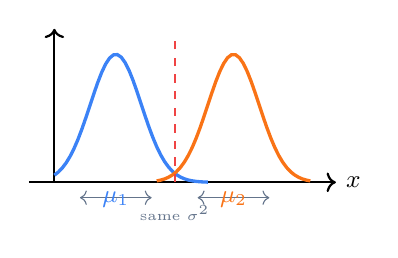
\begin{tikzpicture}[scale=0.65]
  \draw[->, thick] (-0.5,0) -- (5.5,0) node[right] {\small $x$};
  \draw[->, thick] (0,0) -- (0,3);
  % Two Gaussians with same width
  \draw[accent, very thick, domain=0:3, samples=40] plot (\x, {2.5*exp(-2*(\x-1.2)*(\x-1.2))});
  \draw[orange, very thick, domain=2:5, samples=40] plot (\x, {2.5*exp(-2*(\x-3.5)*(\x-3.5))});
  % Same variance arrows
  \draw[<->, muted] (0.5, -0.3) -- (1.9, -0.3);
  \draw[<->, muted] (2.8, -0.3) -- (4.2, -0.3);
  \node[muted] at (2.35, -0.6) {\tiny same $\sigma^2$};
  % Means
  \node[accent, below] at (1.2, 0) {\small $\mu_1$};
  \node[orange, below] at (3.5, 0) {\small $\mu_2$};
  % Decision
  \draw[softred, thick, dashed] (2.35, 0) -- (2.35, 2.8);
\end{tikzpicture}
\end{columns}
\end{frame}


\begin{frame}{LDA: Worked Example ($p = 1$, $K = 2$)}

\begin{columns}
\column{0.48\textwidth}
\textbf{Data:}

Class 1: $n_1 = 30$, $\hat{\mu}_1 = 2$

Class 2: $n_2 = 20$, $\hat{\mu}_2 = 5$

$\hat{\sigma}^2 = 1.5$, $n = 50$

\vspace{0.3em}
$\hat{\pi}_1 = 30/50 = 0.6$

$\hat{\pi}_2 = 20/50 = 0.4$

\column{0.48\textwidth}
\textbf{Discriminant functions:}

$\hat{\delta}_1(x) = x \cdot \dfrac{2}{1.5} - \dfrac{4}{3} + \log(0.6)$

$= 1.33x - 1.33 - 0.51 = 1.33x - 1.84$

\vspace{0.3em}
$\hat{\delta}_2(x) = x \cdot \dfrac{5}{1.5} - \dfrac{25}{3} + \log(0.4)$

$= 3.33x - 8.33 - 0.92 = 3.33x - 9.25$
\end{columns}

\vspace{0.5em}
\textbf{Boundary:} Set $\hat{\delta}_1(x) = \hat{\delta}_2(x)$:
$$1.33x - 1.84 = 3.33x - 9.25 \quad\Rightarrow\quad x = 3.71$$

Classify to Class 1 if $x < 3.71$, Class 2 if $x > 3.71$
\end{frame}


\begin{frame}{LDA with $p > 1$: Multivariate}

\textbf{Assumption:} $X \mid Y = k \;\sim\; N(\boldsymbol{\mu}_k, \boldsymbol{\Sigma})$

$$\delta_k(x) = x^T \boldsymbol{\Sigma}^{-1} \boldsymbol{\mu}_k - \frac{1}{2}\boldsymbol{\mu}_k^T \boldsymbol{\Sigma}^{-1} \boldsymbol{\mu}_k + \log(\pi_k)$$

\begin{columns}
\column{0.5\textwidth}
\textbf{Key points:}
\begin{itemize}
  \item \textbf{Common} covariance $\boldsymbol{\Sigma}$ for all classes
  \item Decision boundary is \textbf{linear} (hyperplane)
  \item Estimates: $\hat{\boldsymbol{\mu}}_k$, $\hat{\boldsymbol{\Sigma}}$, $\hat{\pi}_k$
  \item R: \texttt{MASS::lda(y \textasciitilde{} x1 + x2)}
\end{itemize}

\column{0.45\textwidth}
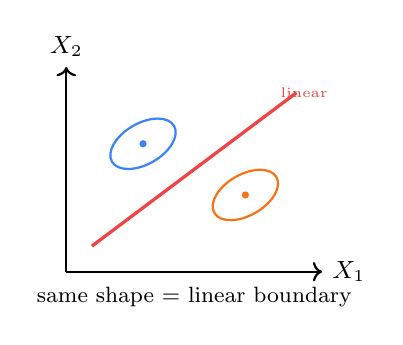
\begin{tikzpicture}[scale=0.65]
  \draw[->, thick] (0,0) -- (5,0) node[right] {\small $X_1$};
  \draw[->, thick] (0,0) -- (0,4) node[above] {\small $X_2$};
  % Class 1 ellipse
  \draw[accent, thick, rotate around={30:(1.5,2.5)}] (1.5,2.5) ellipse (0.7 and 0.4);
  \fill[accent] (1.5,2.5) circle (2pt);
  % Class 2 ellipse
  \draw[orange, thick, rotate around={30:(3.5,1.5)}] (3.5,1.5) ellipse (0.7 and 0.4);
  \fill[orange] (3.5,1.5) circle (2pt);
  % Linear boundary
  \draw[softred, very thick] (0.5, 0.5) -- (4.5, 3.5);
  \node[softred, right] at (4, 3.5) {\tiny linear};
  \node at (2.5, -0.5) {\footnotesize same shape = linear boundary};
\end{tikzpicture}
\end{columns}
\end{frame}


% ═══════════ QDA ═══════════
\begin{frame}{Quadratic Discriminant Analysis (QDA)}

\textbf{Relaxation:} Each class has its \textbf{own} covariance matrix $\boldsymbol{\Sigma}_k$

$$\delta_k(x) = -\frac{1}{2}(x - \mu_k)^T \boldsymbol{\Sigma}_k^{-1}(x - \mu_k) - \frac{1}{2}\log|\boldsymbol{\Sigma}_k| + \log \pi_k$$

\begin{columns}
\column{0.5\textwidth}
Decision boundary is \textbf{quadratic} (curved)

\vspace{0.3em}
\textbf{Bias-Variance:}
\begin{itemize}
  \item LDA: $Kp$ parameters (lower variance)
  \item QDA: $Kp(p+1)/2$ parameters (more flexible)
\end{itemize}

\vspace{0.3em}
QDA better when classes truly have\\different covariance structures

\column{0.45\textwidth}
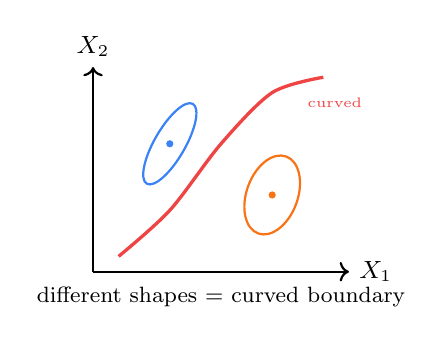
\begin{tikzpicture}[scale=0.65]
  \draw[->, thick] (0,0) -- (5,0) node[right] {\small $X_1$};
  \draw[->, thick] (0,0) -- (0,4) node[above] {\small $X_2$};
  % Class 1 ellipse (narrow)
  \draw[accent, thick, rotate around={60:(1.5,2.5)}] (1.5,2.5) ellipse (0.9 and 0.3);
  \fill[accent] (1.5,2.5) circle (2pt);
  % Class 2 ellipse (wide)
  \draw[orange, thick, rotate around={-20:(3.5,1.5)}] (3.5,1.5) ellipse (0.5 and 0.8);
  \fill[orange] (3.5,1.5) circle (2pt);
  % Curved boundary
  \draw[softred, very thick, smooth, tension=0.5] plot coordinates {(0.5,0.3)(1.5,1.2)(2.5,2.5)(3.5,3.5)(4.5,3.8)};
  \node[softred, right] at (4, 3.3) {\tiny curved};
  \node at (2.5, -0.5) {\footnotesize different shapes = curved boundary};
\end{tikzpicture}
\end{columns}
\end{frame}


\begin{frame}{LDA vs.\ QDA: When to Use Which?}

\begin{center}
\begin{tabular}{lcc}
\toprule
Feature & LDA & QDA \\
\midrule
Covariance & Common $\boldsymbol{\Sigma}$ & Class-specific $\boldsymbol{\Sigma}_k$ \\
Boundary & Linear & Quadratic \\
\# Parameters & $Kp$ & $Kp(p+1)/2$ \\
Variance & Lower & Higher \\
Bias & Higher & Lower \\
Best when & Small $n$, similar classes & Large $n$, different shapes \\
\bottomrule
\end{tabular}
\end{center}

\vspace{0.5em}
\centering
\textit{Same bias-variance trade-off as always!}

\vspace{0.3em}
R: \texttt{MASS::lda(...)} \quad vs \quad \texttt{MASS::qda(...)}
\end{frame}


% ═══════════ NAIVE BAYES ═══════════
\begin{frame}{Naive Bayes Classifier}

\textbf{Key assumption:} Predictors are \textbf{independent} within each class

$$f_k(x) = \prod_{j=1}^{p} f_{kj}(x_j)$$

\begin{columns}
\column{0.5\textwidth}
\textbf{Why ``naive''?}

Independence is almost never true!

But it works surprisingly well in practice

\vspace{0.5em}
\textbf{Advantage:}
\begin{itemize}
  \item Estimate $p$ one-dimensional densities\\instead of one $p$-dimensional density
  \item Works well with large $p$
  \item Very fast
\end{itemize}

\column{0.45\textwidth}
\textbf{Options for $f_{kj}$:}

\vspace{0.3em}
\begin{tabular}{ll}
\toprule
$X_j$ type & $f_{kj}$ \\
\midrule
Quantitative & Gaussian \\
Quantitative & Kernel density \\
Qualitative & Frequency table \\
\bottomrule
\end{tabular}

\vspace{0.5em}
R: \texttt{e1071::naiveBayes(...)}
\end{columns}
\end{frame}


% ═══════════ KNN ═══════════
\begin{frame}{KNN for Classification (Revisited)}
\begin{columns}
\column{0.5\textwidth}
$$P(Y = k \mid X = x_0) = \frac{1}{K}\sum_{i \in \mathcal{N}_0} \mathbf{1}(y_i = k)$$

\vspace{0.3em}
\textbf{No model assumptions at all!}

\begin{itemize}
  \item Completely non-parametric
  \item $K$ controls flexibility
  \item Decision boundary can be very complex
  \item Struggles with large $p$ (curse of dimensionality)
\end{itemize}

\column{0.45\textwidth}
\textbf{Smarket data:} KNN results

\vspace{0.3em}
\begin{tabular}{cc}
\toprule
$K$ & Test accuracy \\
\midrule
1 & 50.0\% \\
3 & 53.2\% \\
5 & 51.6\% \\
10 & 52.0\% \\
\bottomrule
\end{tabular}

\vspace{0.3em}
Not great! Stock data is very noisy

\vspace{0.3em}
\footnotesize R: \texttt{class::knn(...)}
\end{columns}
\end{frame}


% ═══════════ COMPARISON ═══════════
\begin{frame}{Comparing All Five Methods}

\begin{center}
\begin{tabular}{lccccc}
\toprule
 & Logistic & LDA & QDA & NB & KNN \\
\midrule
Boundary & linear & linear & quadratic & depends & flexible \\
Assumptions & logit linear & Gaussian, $\Sigma$ & Gaussian, $\Sigma_k$ & independence & none \\
\# Params & $p+1$ & $Kp$ & $Kp^2/2$ & $Kp$ & 0 \\
Interpretable & \textcolor{softgreen}{\checkmark\checkmark} & \textcolor{softgreen}{\checkmark} & $\sim$ & $\sim$ & \textcolor{softred}{$\times$} \\
Large $p$ & good & good & risky & \textcolor{softgreen}{great} & \textcolor{softred}{bad} \\
\bottomrule
\end{tabular}
\end{center}

\vspace{0.5em}
\textbf{Rule of thumb:}
\begin{itemize}
  \item Linear boundary true? $\Rightarrow$ Logistic $\approx$ LDA
  \item Moderate non-linearity? $\Rightarrow$ QDA or Naive Bayes
  \item Small $p$, large $n$, complex boundary? $\Rightarrow$ KNN
\end{itemize}
\end{frame}


\begin{frame}{When Does Each Method Win?}

\begin{center}
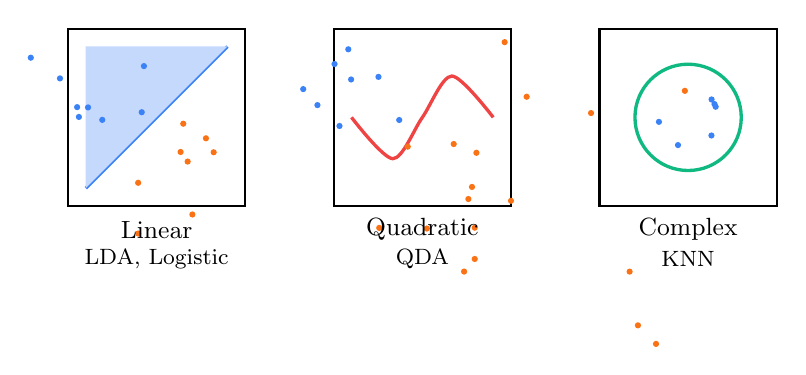
\begin{tikzpicture}[scale=0.75]
  % Scenario 1
  \begin{scope}[xshift=0cm]
    \draw[thick] (0,0) rectangle (3,3);
    \draw[accent, very thick] (0.3, 0.3) -- (2.7, 2.7);
    \fill[accent!30] (0.3,2.7) -- (0.3,0.3) -- (2.7,2.7) -- cycle;
    \foreach \i in {1,...,8} {
      \pgfmathsetmacro{\x}{0.3+rand*1.1}
      \pgfmathsetmacro{\y}{1.8+rand*0.8}
      \fill[accent] (\x,\y) circle (1.5pt);
    }
    \foreach \i in {1,...,8} {
      \pgfmathsetmacro{\x}{1.8+rand*0.8}
      \pgfmathsetmacro{\y}{0.3+rand*1.1}
      \fill[orange] (\x,\y) circle (1.5pt);
    }
    \node at (1.5, -0.4) {\small Linear};
    \node at (1.5, -0.9) {\footnotesize LDA, Logistic};
  \end{scope}

  % Scenario 2
  \begin{scope}[xshift=4.5cm]
    \draw[thick] (0,0) rectangle (3,3);
    \draw[softred, very thick, smooth, tension=0.5] plot coordinates {(0.3,1.5)(1,0.8)(1.5,1.5)(2,2.2)(2.7,1.5)};
    \foreach \i in {1,...,8} {
      \pgfmathsetmacro{\x}{0.3+rand*1.1}
      \pgfmathsetmacro{\y}{2+rand*0.7}
      \fill[accent] (\x,\y) circle (1.5pt);
    }
    \foreach \i in {1,...,8} {
      \pgfmathsetmacro{\x}{1.5+rand*1}
      \pgfmathsetmacro{\y}{0.3+rand*0.8}
      \fill[orange] (\x,\y) circle (1.5pt);
    }
    \node at (1.5, -0.4) {\small Quadratic};
    \node at (1.5, -0.9) {\footnotesize QDA};
  \end{scope}

  % Scenario 3
  \begin{scope}[xshift=9cm]
    \draw[thick] (0,0) rectangle (3,3);
    \draw[softgreen, very thick] (1.5,1.5) circle (0.9);
    \foreach \i in {1,...,6} {
      \pgfmathsetmacro{\a}{rand*360}
      \pgfmathsetmacro{\x}{1.5+0.5*cos(\a)}
      \pgfmathsetmacro{\y}{1.5+0.5*sin(\a)}
      \fill[accent] (\x,\y) circle (1.5pt);
    }
    \foreach \i in {1,...,10} {
      \pgfmathsetmacro{\x}{0.2+rand*2.6}
      \pgfmathsetmacro{\y}{0.2+rand*2.6}
      \fill[orange] (\x,\y) circle (1.5pt);
    }
    \node at (1.5, -0.4) {\small Complex};
    \node at (1.5, -0.9) {\footnotesize KNN};
  \end{scope}
\end{tikzpicture}
\end{center}
\end{frame}


\begin{frame}{Smarket Data: Method Comparison}

\textbf{S\&P 500 daily returns:} Predict Up/Down using Lag1, Lag2

Train: 2001--2004 \quad Test: 2005

\vspace{0.3em}
\begin{center}
\begin{tabular}{lcc}
\toprule
Method & Test Accuracy & Note \\
\midrule
Logistic Regression & 56.1\% & best linear method \\
LDA & 56.0\% & almost identical \\
QDA & 59.9\% & \textcolor{softgreen}{best overall} \\
Naive Bayes & 59.0\% & close to QDA \\
KNN ($K=1$) & 50.0\% & random coin flip \\
\bottomrule
\end{tabular}
\end{center}

\vspace{0.3em}
QDA wins $\Rightarrow$ evidence of non-linear decision boundary

Logistic $\approx$ LDA $\Rightarrow$ both produce linear boundaries

KNN overfits badly with $K=1$
\end{frame}


% ═══════════ ADDITIONAL CONCEPT SLIDES ═══════════
\begin{frame}{Logistic Regression: Interpreting Coefficients}

\begin{columns}
\column{0.5\textwidth}
$\hat{\beta}_1 = 0.0055$ (balance)

\vspace{0.3em}
\textbf{Odds ratio:}

$$e^{\hat{\beta}_1} = e^{0.0055} = 1.0055$$

A \$1 increase in balance multiplies\\
the odds of default by $1.0055$

\vspace{0.3em}
A \$100 increase:

$e^{0.0055 \times 100} = e^{0.55} = 1.73$

\textcolor{accent}{Odds increase by 73\%!}

\column{0.45\textwidth}
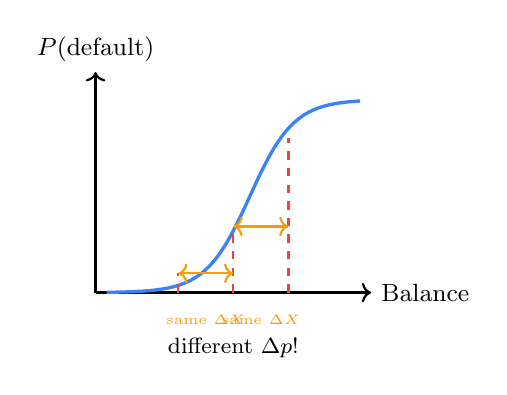
\begin{tikzpicture}[scale=0.7]
  \draw[->, thick] (0,0) -- (5,0) node[right] {\small Balance};
  \draw[->, thick] (0,0) -- (0,4) node[above] {\small $P(\text{default})$};
  \draw[accent, very thick, domain=0.2:4.8, samples=50] plot (\x, {3.5/(1+exp(-2.5*(\x-2.8)))});
  % Show non-linearity
  \draw[softred, thick, dashed] (1.5, 0) -- (1.5, 0.35);
  \draw[softred, thick, dashed] (2.5, 0) -- (2.5, 1.2);
  \draw[softred, thick, dashed] (3.5, 0) -- (3.5, 2.8);
  \draw[<->, amber, thick] (1.5, 0.35) -- (2.5, 0.35);
  \draw[<->, amber, thick] (2.5, 1.2) -- (3.5, 1.2);
  \node[amber] at (2, -0.5) {\tiny same $\Delta X$};
  \node[amber] at (3, -0.5) {\tiny same $\Delta X$};
  \node at (2.5, -1) {\footnotesize different $\Delta p$!};
\end{tikzpicture}
\end{columns}
\end{frame}


\begin{frame}{Why LDA and Logistic Give Similar Results}

\begin{columns}
\column{0.55\textwidth}
\textbf{Both produce linear decision boundaries}

\vspace{0.3em}
LDA: assumes Gaussian classes with $\boldsymbol{\Sigma}$ shared

Logistic: directly models log-odds as linear

\vspace{0.5em}
\textbf{When they differ:}
\begin{itemize}
  \item LDA better if Gaussian assumption holds
  \item Logistic more robust to non-Gaussian data
  \item LDA uses full density $\Rightarrow$ more efficient if correct
  \item Logistic uses only boundary $\Rightarrow$ more robust
\end{itemize}

\column{0.4\textwidth}
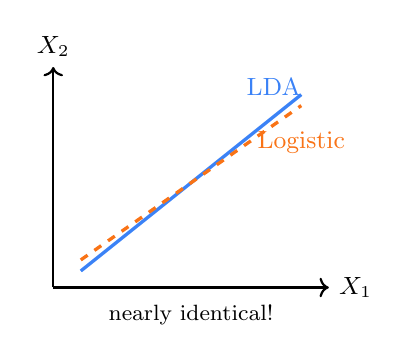
\begin{tikzpicture}[scale=0.7]
  \draw[->, thick] (0,0) -- (5,0) node[right] {\small $X_1$};
  \draw[->, thick] (0,0) -- (0,4) node[above] {\small $X_2$};
  % LDA boundary
  \draw[accent, very thick] (0.5, 0.3) -- (4.5, 3.5);
  \node[accent, above] at (4, 3.3) {\small LDA};
  % Logistic boundary (nearly identical)
  \draw[orange, very thick, dashed] (0.5, 0.5) -- (4.5, 3.3);
  \node[orange, below] at (4.5, 3.0) {\small Logistic};
  \node at (2.5, -0.5) {\footnotesize nearly identical!};
\end{tikzpicture}
\end{columns}
\end{frame}


\begin{frame}{Multiclass Logistic: Softmax}

For $K > 2$ classes:

$$P(Y = k \mid X) = \frac{e^{\beta_{k0} + \beta_{k1}X_1 + \cdots + \beta_{kp}X_p}}{\sum_{l=1}^{K} e^{\beta_{l0} + \beta_{l1}X_1 + \cdots + \beta_{lp}X_p}}$$

\begin{columns}
\column{0.5\textwidth}
\begin{itemize}
  \item Each class $k$ has its own coefficient vector $\boldsymbol{\beta}_k$
  \item Probabilities sum to 1 across classes
  \item Called \textbf{softmax} function
  \item Used heavily in deep learning (Week 9)
\end{itemize}

\column{0.45\textwidth}
\textbf{Example:} $K = 3$ classes

$p_1 = 0.6$, $p_2 = 0.3$, $p_3 = 0.1$

$\sum = 1.0$ \textcolor{softgreen}{\checkmark}

\vspace{0.3em}
Classify to Class 1
\end{columns}
\end{frame}


\begin{frame}{Poisson Regression: Count Data}

$$\log(\lambda(X)) = \beta_0 + \beta_1 X_1 + \cdots + \beta_p X_p$$

where $Y \sim \text{Poisson}(\lambda)$

\begin{columns}
\column{0.5\textwidth}
\textbf{When to use:}
\begin{itemize}
  \item Response is a \textbf{count} (0, 1, 2, \ldots)
  \item Examples: \# bike rentals, \# ER visits
  \item Cannot be negative
\end{itemize}

\vspace{0.3em}
\textbf{Bikeshare data:}

\texttt{bikers \textasciitilde{} hr + temp + weathersit}

\column{0.45\textwidth}
\textbf{Generalized Linear Models:}

\begin{tabular}{ll}
\toprule
Response & Link \\
\midrule
Continuous & identity (OLS) \\
Binary & logit (logistic) \\
Count & log (Poisson) \\
\bottomrule
\end{tabular}

\vspace{0.3em}
\footnotesize R: \texttt{glm(..., family = poisson)}

All are special cases of GLMs!
\end{columns}
\end{frame}


\begin{frame}{Prior Probabilities Matter}

\begin{columns}
\column{0.55\textwidth}
\textbf{LDA uses $\pi_k$} in the discriminant function:

$$\delta_k(x) = x \cdot \frac{\mu_k}{\sigma^2} - \frac{\mu_k^2}{2\sigma^2} + \textcolor{softred}{\log(\pi_k)}$$

\vspace{0.3em}
If $\pi_1 \gg \pi_2$: boundary shifts\\
toward Class 2

\vspace{0.3em}
\textbf{Imbalanced classes:}

Default rate $= 3.3\%$

$\pi_{\text{No}} = 0.967$, $\pi_{\text{Yes}} = 0.033$

\vspace{0.2em}
LDA is biased toward ``No''

\column{0.4\textwidth}
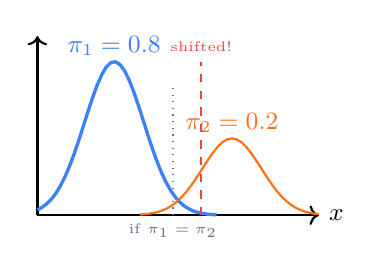
\begin{tikzpicture}[scale=0.65]
  \draw[->, thick] (0,0) -- (5.5,0) node[right] {\small $x$};
  \draw[->, thick] (0,0) -- (0,3.5);
  % Class 1 (large prior)
  \draw[accent, very thick, domain=0:3.5, samples=40] plot (\x, {3*exp(-1.5*(\x-1.5)*(\x-1.5))});
  \node[accent] at (1.5, 3.3) {\small $\pi_1 = 0.8$};
  % Class 2 (small prior)
  \draw[orange, thick, domain=2:5.5, samples=40] plot (\x, {1.5*exp(-1.5*(\x-3.8)*(\x-3.8))});
  \node[orange] at (3.8, 1.8) {\small $\pi_2 = 0.2$};
  % Boundary shifts right
  \draw[softred, thick, dashed] (3.2, 0) -- (3.2, 3);
  \node[softred, above] at (3.2, 3) {\tiny shifted!};
  % Equal prior boundary
  \draw[muted, dotted] (2.65, 0) -- (2.65, 2.5);
  \node[muted] at (2.65, -0.3) {\tiny if $\pi_1 = \pi_2$};
\end{tikzpicture}
\end{columns}
\end{frame}


\begin{frame}{Sensitivity vs.\ Specificity: The Trade-Off}

\begin{center}
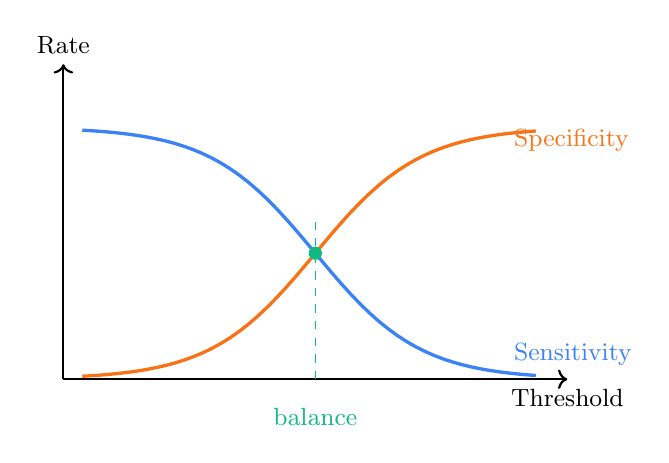
\begin{tikzpicture}[scale=0.8]
  \draw[->, thick] (0,0) -- (8,0) node[below] {\small Threshold};
  \draw[->, thick] (0,0) -- (0,5) node[above] {\small Rate};

  % Sensitivity
  \draw[accent, very thick, domain=0.3:7.5, samples=50] plot (\x, {4/(1+exp(1.2*(\x-4)))});
  \node[accent, right] at (7, 0.4) {\small Sensitivity};

  % Specificity
  \draw[orange, very thick, domain=0.3:7.5, samples=50] plot (\x, {4/(1+exp(-1.2*(\x-4)))});
  \node[orange, right] at (7, 3.8) {\small Specificity};

  % Optimal
  \draw[softgreen, dashed] (4, 0) -- (4, 2.5);
  \fill[softgreen] (4, 2) circle (3pt);
  \node[softgreen, below] at (4, -0.3) {\small balance};
\end{tikzpicture}
\end{center}

As threshold $\uparrow$: sensitivity $\downarrow$, specificity $\uparrow$

The ROC curve traces this entire trade-off
\end{frame}


\begin{frame}{Practical Workflow for Classification}

\begin{center}
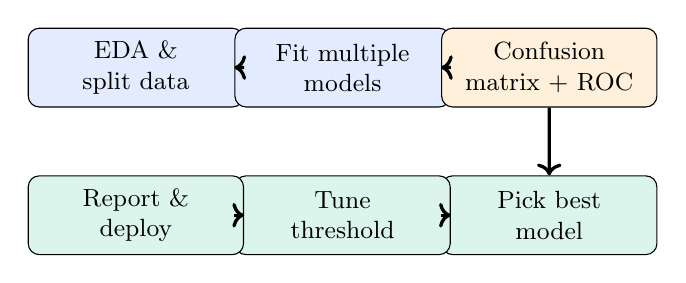
\begin{tikzpicture}[scale=0.75, every node/.style={font=\small, text width=2.5cm, align=center}]
  \node[draw, fill=accent!15, rounded corners, minimum height=1cm] (eda) at (0,3) {EDA \&\\split data};
  \node[draw, fill=accent!15, rounded corners, minimum height=1cm] (fit) at (3.5,3) {Fit multiple\\models};
  \node[draw, fill=amber!15, rounded corners, minimum height=1cm] (eval) at (7,3) {Confusion\\matrix + ROC};
  \node[draw, fill=softgreen!15, rounded corners, minimum height=1cm] (pick) at (7,0.5) {Pick best\\model};
  \node[draw, fill=softgreen!15, rounded corners, minimum height=1cm] (thresh) at (3.5,0.5) {Tune\\threshold};
  \node[draw, fill=softgreen!15, rounded corners, minimum height=1cm] (report) at (0,0.5) {Report \&\\deploy};

  \draw[->, very thick] (eda) -- (fit);
  \draw[->, very thick] (fit) -- (eval);
  \draw[->, very thick] (eval) -- (pick);
  \draw[->, very thick] (pick) -- (thresh);
  \draw[->, very thick] (thresh) -- (report);
\end{tikzpicture}
\end{center}

\vspace{0.3em}
\textbf{Always compare:} Logistic, LDA, QDA, KNN on the same test set!
\end{frame}


\begin{frame}{R Functions: Quick Reference}

\begin{center}
\begin{tabular}{ll}
\toprule
\texttt{glm(y \textasciitilde{} x, family = binomial)} & Logistic regression \\
\texttt{predict(fit, type = "response")} & Predicted probabilities \\
\texttt{MASS::lda(y \textasciitilde{} x, data)} & Linear discriminant analysis \\
\texttt{MASS::qda(y \textasciitilde{} x, data)} & Quadratic discriminant analysis \\
\texttt{e1071::naiveBayes(y \textasciitilde{} x)} & Naive Bayes \\
\texttt{class::knn(train, test, cl, k)} & K-nearest neighbors \\
\texttt{table(predicted, actual)} & Confusion matrix \\
\bottomrule
\end{tabular}
\end{center}

\vspace{0.5em}
\begin{center}
\begin{tabular}{ll}
\toprule
\texttt{contrasts(factor\_var)} & See dummy variable coding \\
\texttt{predict(lda.fit)\$posterior} & Posterior probabilities \\
\texttt{predict(lda.fit)\$class} & Predicted classes \\
\bottomrule
\end{tabular}
\end{center}
\end{frame}


\begin{frame}{Key Formulas: Cheat Sheet}
\begin{columns}
\column{0.48\textwidth}
\textbf{Logistic Regression:}
\begin{align*}
p(X) &= \frac{e^{\beta_0 + \beta_1 X}}{1 + e^{\beta_0 + \beta_1 X}} \\[4pt]
\text{logit}(p) &= \log\frac{p}{1-p} = \beta_0 + \beta_1 X
\end{align*}

\textbf{LDA ($p = 1$):}
$$\delta_k(x) = x\frac{\mu_k}{\sigma^2} - \frac{\mu_k^2}{2\sigma^2} + \log \pi_k$$

\column{0.48\textwidth}
\textbf{Bayes' Theorem:}
$$P(Y=k \mid X) = \frac{\pi_k f_k(x)}{\sum_l \pi_l f_l(x)}$$

\textbf{Evaluation:}
\begin{align*}
\text{Sens.} &= \text{TP} / (\text{TP} + \text{FN}) \\
\text{Spec.} &= \text{TN} / (\text{TN} + \text{FP}) \\
\text{Prec.} &= \text{TP} / (\text{TP} + \text{FP})
\end{align*}
\end{columns}
\end{frame}


% ═══════════ ADDITIONAL DEEP-DIVE SLIDES ═══════════

\begin{frame}{Think About It: Why Does the Sigmoid Work?}
\begin{columns}
\column{0.5\textwidth}
\textbf{We need:} $p(X) \in (0, 1)$

\vspace{0.3em}
Start with linear predictor:\\
$z = \beta_0 + \beta_1 X \in (-\infty, +\infty)$

\vspace{0.3em}
Apply sigmoid: $\sigma(z) = \dfrac{e^z}{1 + e^z}$

\vspace{0.3em}
\begin{tabular}{cc}
\toprule
$z$ & $\sigma(z)$ \\
\midrule
$-\infty$ & $0$ \\
$-2$ & $0.12$ \\
$0$ & $0.50$ \\
$+2$ & $0.88$ \\
$+\infty$ & $1$ \\
\bottomrule
\end{tabular}

\column{0.45\textwidth}
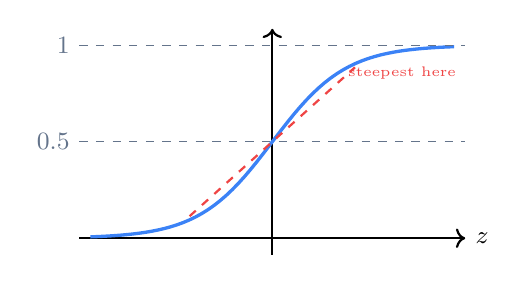
\begin{tikzpicture}[scale=0.7]
  \draw[->, thick] (-3.5,0) -- (3.5,0) node[right] {\small $z$};
  \draw[->, thick] (0,-0.3) -- (0,3.8);
  % Sigmoid
  \draw[accent, very thick, domain=-3.3:3.3, samples=60] plot (\x, {3.5/(1+exp(-1.5*\x))});
  % Labels
  \draw[muted, dashed] (-3.5, 3.5) -- (3.5, 3.5);
  \node[muted, left] at (-3.5, 3.5) {\small $1$};
  \draw[muted, dashed] (-3.5, 1.75) -- (3.5, 1.75);
  \node[muted, left] at (-3.5, 1.75) {\small $0.5$};
  % Slope at 0
  \draw[softred, thick, dashed] (-1.5, 0.4) -- (1.5, 3.1);
  \node[softred, right] at (1.2, 3.0) {\tiny steepest here};
\end{tikzpicture}

\vspace{0.3em}
\textit{Smoothly maps $\mathbb{R} \to (0,1)$}
\end{columns}
\end{frame}


\begin{frame}{Worked Example: Will This Customer Default?}

\textbf{Model:} $\log\left(\frac{p}{1-p}\right) = -10.65 + 0.0055 \cdot \text{balance}$

\vspace{0.3em}
\begin{columns}
\column{0.48\textwidth}
\textbf{Customer A:} balance = \$500

$z = -10.65 + 0.0055 \times 500 = -7.90$

$p = \sigma(-7.90) = 0.0004$

\textcolor{softgreen}{$0.04\%$ chance --- safe!}

\vspace{0.5em}
\textbf{Customer B:} balance = \$1,500

$z = -10.65 + 0.0055 \times 1500 = -2.40$

$p = \sigma(-2.40) = 0.083$

\textcolor{amber}{$8.3\%$ chance --- watch closely}

\column{0.48\textwidth}
\textbf{Customer C:} balance = \$2,000

$z = -10.65 + 0.0055 \times 2000 = 0.35$

$p = \sigma(0.35) = 0.587$

\textcolor{softred}{$58.7\%$ chance --- likely default!}

\vspace{0.5em}
\textbf{Customer D:} balance = \$2,500

$z = -10.65 + 0.0055 \times 2500 = 3.10$

$p = \sigma(3.10) = 0.957$

\textcolor{softred}{\textbf{95.7\%} --- almost certain default}
\end{columns}
\end{frame}


\begin{frame}{The Confounding Story: Student Status}

\begin{columns}
\column{0.48\textwidth}
\textbf{Simple logistic:}

default $\sim$ student

$\hat{\beta}_{\text{student}} = +0.40$ $(p < 0.001)$

Students default \textit{more}!

\vspace{0.5em}
\textbf{Multiple logistic:}

default $\sim$ balance + student

$\hat{\beta}_{\text{student}} = -0.65$ $(p < 0.001)$

Students default \textit{less}!

\column{0.48\textwidth}
\textbf{The explanation:}

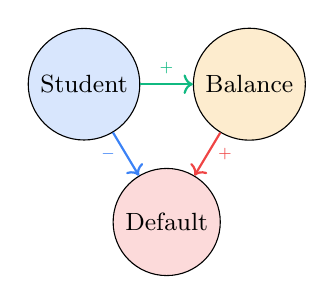
\begin{tikzpicture}[scale=0.7]
  \node[draw, circle, fill=accent!20, minimum size=1.2cm, font=\small] (s) at (0, 2.5) {Student};
  \node[draw, circle, fill=amber!20, minimum size=1.2cm, font=\small] (b) at (3, 2.5) {Balance};
  \node[draw, circle, fill=softred!20, minimum size=1.2cm, font=\small] (d) at (1.5, 0) {Default};
  \draw[->, thick, softgreen] (s) -- (b) node[midway, above] {\tiny $+$};
  \draw[->, thick, softred] (b) -- (d) node[midway, right] {\tiny $+$};
  \draw[->, thick, accent] (s) -- (d) node[midway, left] {\tiny $-$};
\end{tikzpicture}

\vspace{0.3em}
Students carry higher balances\\
but at same balance, they're more\\
responsible $\Rightarrow$ lower default
\end{columns}
\end{frame}


\begin{frame}{Maximum Likelihood: Why Not Least Squares?}

\begin{columns}
\column{0.5\textwidth}
\textbf{Least squares:}
\begin{itemize}
  \item Minimizes $\sum(y_i - p(x_i))^2$
  \item Works, but is not optimal
  \item Can give multiple solutions
  \item Non-convex optimization
\end{itemize}

\vspace{0.3em}
\textbf{Maximum likelihood:}
\begin{itemize}
  \item Maximizes $\prod p_i^{y_i}(1-p_i)^{1-y_i}$
  \item Unique global maximum
  \item Convex (in log-likelihood)
  \item Statistically efficient
\end{itemize}

\column{0.45\textwidth}
\textbf{Log-likelihood:}

$$\ell = \sum_{i=1}^{n} \left[ y_i \log p_i + (1-y_i) \log(1-p_i) \right]$$

This is also called \textbf{cross-entropy loss}

\vspace{0.5em}
Used everywhere in deep learning!

\vspace{0.3em}
\textit{MLE and cross-entropy are the\\same thing with different names}
\end{columns}
\end{frame}


\begin{frame}{LDA: The Geometry}
\begin{columns}
\column{0.55\textwidth}
\textbf{What LDA actually does:}

\begin{enumerate}
  \item Project data onto the direction that \textbf{maximizes} separation between class means
  \item While \textbf{minimizing} within-class variance
  \item This direction is $\boldsymbol{\Sigma}^{-1}(\boldsymbol{\mu}_1 - \boldsymbol{\mu}_2)$
\end{enumerate}

\vspace{0.3em}
Fisher's criterion:
$$J = \frac{(\mu_1 - \mu_2)^2}{\sigma_1^2 + \sigma_2^2}$$

Maximize between-class / within-class

\column{0.4\textwidth}
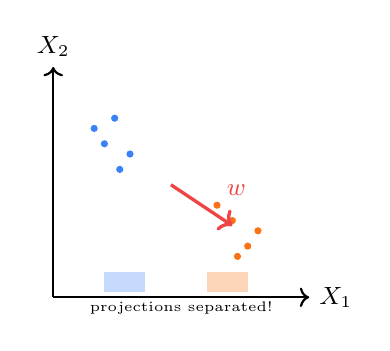
\begin{tikzpicture}[scale=0.65]
  \draw[->, thick] (0,0) -- (5,0) node[right] {\small $X_1$};
  \draw[->, thick] (0,0) -- (0,4.5) node[above] {\small $X_2$};
  % Class 1
  \foreach \x/\y in {1/3, 1.3/2.5, 0.8/3.3, 1.5/2.8, 1.2/3.5} {
    \fill[accent] (\x,\y) circle (2pt);
  }
  % Class 2
  \foreach \x/\y in {3.5/1.5, 3.8/1, 3.2/1.8, 4/1.3, 3.6/0.8} {
    \fill[orange] (\x,\y) circle (2pt);
  }
  % Projection direction
  \draw[softred, very thick, ->] (2.3, 2.2) -- (3.5, 1.4);
  \node[softred, above right] at (3.2, 1.8) {\small $w$};
  % Projected distributions
  \draw[accent, thick] (1, 0.3) -- (1.8, 0.3);
  \fill[accent!30] (1, 0.1) rectangle (1.8, 0.5);
  \draw[orange, thick] (3, 0.3) -- (3.8, 0.3);
  \fill[orange!30] (3, 0.1) rectangle (3.8, 0.5);
  \node at (2.5, -0.2) {\tiny projections separated!};
\end{tikzpicture}
\end{columns}
\end{frame}


\begin{frame}{LDA for $K = 3$ Classes: Worked Example}

\textbf{Three types of iris flowers:} Setosa, Versicolor, Virginica

\begin{columns}
\column{0.5\textwidth}
\begin{tabular}{lccc}
\toprule
 & $n_k$ & $\hat{\mu}_{k1}$ & $\hat{\mu}_{k2}$ \\
\midrule
Setosa & 50 & 5.01 & 3.43 \\
Versicolor & 50 & 5.94 & 2.77 \\
Virginica & 50 & 6.59 & 2.97 \\
\bottomrule
\end{tabular}

Using sepal length ($X_1$) and sepal width ($X_2$)

$\hat{\pi}_k = 1/3$ for all classes

\column{0.45\textwidth}
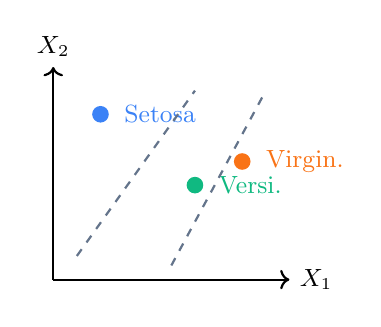
\begin{tikzpicture}[scale=0.6]
  \draw[->, thick] (0,0) -- (5,0) node[right] {\small $X_1$};
  \draw[->, thick] (0,0) -- (0,4.5) node[above] {\small $X_2$};
  % Three class centers
  \fill[accent] (1, 3.5) circle (5pt);
  \node[accent, right] at (1.3, 3.5) {\small Setosa};
  \fill[softgreen] (3, 2) circle (5pt);
  \node[softgreen, right] at (3.3, 2) {\small Versi.};
  \fill[orange] (4, 2.5) circle (5pt);
  \node[orange, right] at (4.3, 2.5) {\small Virgin.};
  % Boundaries
  \draw[muted, thick, dashed] (0.5, 0.5) -- (3, 4);
  \draw[muted, thick, dashed] (2.5, 0.3) -- (4.5, 4);
\end{tikzpicture}

\vspace{0.2em}
Two linear boundaries for 3 classes
\end{columns}
\end{frame}


\begin{frame}{QDA: Worked Numerical Example}

\textbf{Two classes, $p = 1$:}

\begin{columns}
\column{0.48\textwidth}
Class 1: $\hat{\mu}_1 = 2$, $\hat{\sigma}_1^2 = 1$

Class 2: $\hat{\mu}_2 = 5$, $\hat{\sigma}_2^2 = 4$

$\hat{\pi}_1 = \hat{\pi}_2 = 0.5$

\vspace{0.3em}
\textbf{Decision boundary:}

Where $\delta_1(x) = \delta_2(x)$

This gives a \textbf{quadratic} equation in $x$

\column{0.48\textwidth}
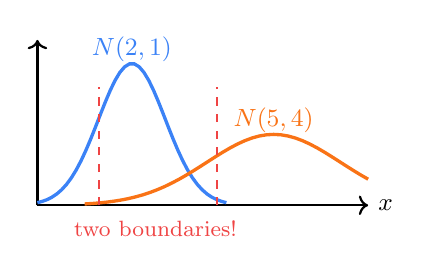
\begin{tikzpicture}[scale=0.6]
  \draw[->, thick] (0,0) -- (7,0) node[right] {\small $x$};
  \draw[->, thick] (0,0) -- (0,3.5);
  % Class 1: narrow
  \draw[accent, very thick, domain=0:4, samples=40] plot (\x, {3*exp(-1*(\x-2)*(\x-2))});
  \node[accent] at (2, 3.3) {\small $N(2, 1)$};
  % Class 2: wide
  \draw[orange, very thick, domain=1:7, samples=40] plot (\x, {1.5*exp(-0.25*(\x-5)*(\x-5))});
  \node[orange] at (5, 1.8) {\small $N(5, 4)$};
  % Boundaries
  \draw[softred, thick, dashed] (1.3, 0) -- (1.3, 2.5);
  \draw[softred, thick, dashed] (3.8, 0) -- (3.8, 2.5);
  \node[softred] at (2.5, -0.5) {\footnotesize two boundaries!};
\end{tikzpicture}

\vspace{0.2em}
\footnotesize Different variances $\Rightarrow$ two crossing points
\end{columns}
\end{frame}


\begin{frame}{Naive Bayes: Worked Example}

\textbf{Spam filter:} Is this email spam?

\begin{columns}
\column{0.5\textwidth}
Features: contains ``free'', ``click'', ``dear''

$\hat{\pi}_{\text{spam}} = 0.4$, $\hat{\pi}_{\text{ham}} = 0.6$

\vspace{0.3em}
\begin{tabular}{lccc}
\toprule
 & free & click & dear \\
\midrule
$P(\cdot \mid \text{spam})$ & 0.8 & 0.7 & 0.1 \\
$P(\cdot \mid \text{ham})$ & 0.1 & 0.1 & 0.5 \\
\bottomrule
\end{tabular}

\vspace{0.3em}
Email has: free=Yes, click=Yes, dear=No

\column{0.45\textwidth}
\textbf{Computation:}

$P(\text{spam}) \times P(\text{free}|\text{spam}) \times P(\text{click}|\text{spam}) \times P(\overline{\text{dear}}|\text{spam})$

$= 0.4 \times 0.8 \times 0.7 \times 0.9 = 0.202$

\vspace{0.3em}
$P(\text{ham}) \times P(\text{free}|\text{ham}) \times P(\text{click}|\text{ham}) \times P(\overline{\text{dear}}|\text{ham})$

$= 0.6 \times 0.1 \times 0.1 \times 0.5 = 0.003$

\vspace{0.3em}
$P(\text{spam} | X) = \frac{0.202}{0.202 + 0.003} = \textcolor{softred}{98.5\%}$

\textcolor{softred}{\textbf{Spam!}}
\end{columns}
\end{frame}


\begin{frame}{Confusion Matrix: Why Accuracy Is Misleading}
\begin{columns}
\column{0.55\textwidth}
\textbf{Disease screening:}

1\% of patients have the disease

\vspace{0.3em}
\textbf{``Always predict healthy'':}

Accuracy = 99\%!

But sensitivity = 0\% --- misses everyone

\vspace{0.5em}
\textbf{Lesson:}

With imbalanced classes, use:
\begin{itemize}
  \item Sensitivity + Specificity
  \item Precision + Recall
  \item F1 score
  \item AUC
\end{itemize}

\column{0.4\textwidth}
\textbf{F1 Score:}

$$F_1 = 2 \cdot \frac{\text{Precision} \times \text{Recall}}{\text{Precision} + \text{Recall}}$$

Harmonic mean of precision \& recall

\vspace{0.5em}
\begin{tabular}{lc}
\toprule
Metric & Value \\
\midrule
Accuracy & 99\% \\
Sensitivity & 0\% \\
F1 & 0\% \\
\bottomrule
\end{tabular}

\vspace{0.3em}
\textcolor{softred}{F1 exposes the problem!}
\end{columns}
\end{frame}


\begin{frame}{ROC Curve: Step-by-Step Construction}

\begin{columns}
\column{0.5\textwidth}
\textbf{For each threshold $t$:}
\begin{enumerate}
  \item Classify: predict ``Yes'' if $\hat{p} \geq t$
  \item Compute TPR (sensitivity)
  \item Compute FPR ($1 -$ specificity)
  \item Plot the point (FPR, TPR)
\end{enumerate}

\vspace{0.3em}
\begin{tabular}{ccc}
\toprule
Threshold & TPR & FPR \\
\midrule
0.1 & 0.95 & 0.40 \\
0.3 & 0.80 & 0.15 \\
0.5 & 0.60 & 0.05 \\
0.7 & 0.30 & 0.01 \\
0.9 & 0.10 & 0.00 \\
\bottomrule
\end{tabular}

\column{0.45\textwidth}
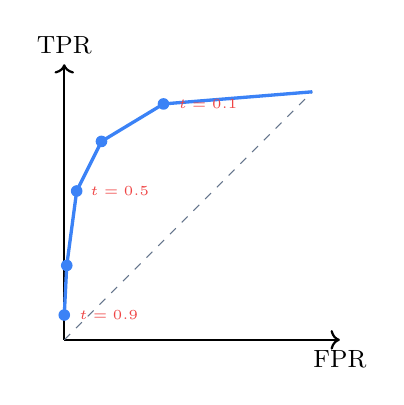
\begin{tikzpicture}[scale=0.7]
  \draw[->, thick] (0,0) -- (5,0) node[below] {\small FPR};
  \draw[->, thick] (0,0) -- (0,5) node[above] {\small TPR};
  \draw[muted, dashed] (0,0) -- (4.5,4.5);
  % ROC points
  \fill[accent] (0, 0.45) circle (3pt);
  \fill[accent] (0.045, 1.35) circle (3pt);
  \fill[accent] (0.225, 2.7) circle (3pt);
  \fill[accent] (0.675, 3.6) circle (3pt);
  \fill[accent] (1.8, 4.28) circle (3pt);
  % Connect
  \draw[accent, very thick] (0, 0.45) -- (0.045, 1.35) -- (0.225, 2.7) -- (0.675, 3.6) -- (1.8, 4.28) -- (4.5, 4.5);
  % Label thresholds
  \node[softred, right, font=\tiny] at (0.1, 0.45) {$t=0.9$};
  \node[softred, right, font=\tiny] at (0.3, 2.7) {$t=0.5$};
  \node[softred, right, font=\tiny] at (1.9, 4.28) {$t=0.1$};
\end{tikzpicture}
\end{columns}
\end{frame}


\begin{frame}{LDA vs.\ Logistic: Same Boundary, Different Path}

\begin{columns}
\column{0.48\textwidth}
\textbf{Logistic (discriminative):}

Models $P(Y \mid X)$ directly

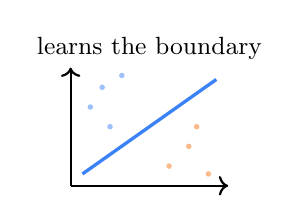
\begin{tikzpicture}[scale=0.5]
  \draw[->, thick] (0,0) -- (4,0);
  \draw[->, thick] (0,0) -- (0,3);
  \node at (2, 3.5) {\small learns the boundary};
  \draw[accent, very thick] (0.3, 0.3) -- (3.7, 2.7);
  \foreach \x/\y in {0.5/2, 0.8/2.5, 1/1.5, 1.3/2.8} { \fill[accent!50] (\x,\y) circle (2pt); }
  \foreach \x/\y in {2.5/0.5, 3/1, 3.5/0.3, 3.2/1.5} { \fill[orange!50] (\x,\y) circle (2pt); }
\end{tikzpicture}

Only cares about the \textbf{boundary}

More robust when Gaussian assumption fails

\column{0.48\textwidth}
\textbf{LDA (generative):}

Models $P(X \mid Y)$ for each class

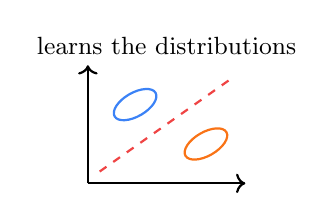
\begin{tikzpicture}[scale=0.5]
  \draw[->, thick] (0,0) -- (4,0);
  \draw[->, thick] (0,0) -- (0,3);
  \node at (2, 3.5) {\small learns the distributions};
  \draw[accent, thick, rotate around={30:(1.2,2)}] (1.2,2) ellipse (0.6 and 0.3);
  \draw[orange, thick, rotate around={30:(3,1)}] (3,1) ellipse (0.6 and 0.3);
  \draw[softred, thick, dashed] (0.3, 0.3) -- (3.7, 2.7);
\end{tikzpicture}

Models the full \textbf{distribution} of each class

More efficient when assumption holds
\end{columns}

\vspace{0.3em}
\centering
\textit{In practice, they almost always give the same answer!}
\end{frame}


\begin{frame}{Number of Parameters: A Practical Guide}

\begin{center}
\begin{tabular}{lcl}
\toprule
Method & \# Parameters & Example: $p=50$, $K=3$ \\
\midrule
Logistic & $(K-1)(p+1)$ & $2 \times 51 = 102$ \\
LDA & $Kp + p(p+1)/2$ & $150 + 1275 = 1425$ \\
QDA & $Kp + Kp(p+1)/2$ & $150 + 3825 = 3975$ \\
Naive Bayes & $2Kp$ & $300$ \\
KNN & $0$ & $0$ \\
\bottomrule
\end{tabular}
\end{center}

\vspace{0.5em}
\textbf{Key insight:}

QDA estimates \textbf{separate} covariance matrices $\Rightarrow$ many parameters

With $p = 50$: QDA needs $\sim 4000$ parameters!

\vspace{0.3em}
$\Rightarrow$ QDA is risky when $n$ is not much larger than $p^2$
\end{frame}


\begin{frame}{The Bias-Variance Trade-Off for Classification}

\begin{center}
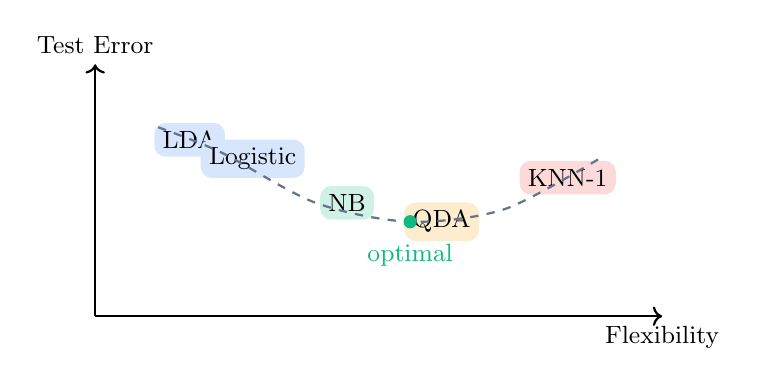
\begin{tikzpicture}[scale=0.8]
  \draw[->, thick] (0,0) -- (9,0) node[below] {\small Flexibility};
  \draw[->, thick] (0,0) -- (0,4) node[above] {\small Test Error};

  % Place methods
  \node[fill=accent!20, rounded corners, inner sep=3pt, font=\small] at (1.5, 2.8) {LDA};
  \node[fill=accent!20, rounded corners, inner sep=3pt, font=\small] at (2.5, 2.5) {Logistic};
  \node[fill=softgreen!20, rounded corners, inner sep=3pt, font=\small] at (4, 1.8) {NB};
  \node[fill=amber!20, rounded corners, inner sep=3pt, font=\small] at (5.5, 1.5) {QDA};
  \node[fill=softred!20, rounded corners, inner sep=3pt, font=\small] at (7.5, 2.2) {KNN-1};

  % U-shape
  \draw[muted, thick, dashed, smooth, tension=0.5] plot coordinates {(1,3)(2,2.6)(3.5,1.8)(5,1.5)(6.5,1.7)(8,2.5)};

  % Optimal
  \fill[softgreen] (5, 1.5) circle (3pt);
  \node[softgreen, below] at (5, 1.3) {\small optimal};
\end{tikzpicture}
\end{center}

Same principle: more flexible $\neq$ always better!
\end{frame}


\begin{frame}{Threshold Selection: A Business Decision}
\begin{columns}
\column{0.55\textwidth}
\textbf{Credit card fraud:}

\begin{tabular}{lcc}
\toprule
 & Cost of FP & Cost of FN \\
\midrule
Fraud & Block card (\$10) & Lose \$5,000 \\
Default & Deny credit (\$200) & Lose \$10,000 \\
Cancer & Biopsy (\$500) & Miss cancer \\
\bottomrule
\end{tabular}

\vspace{0.3em}
\textbf{When FN is expensive:}

Lower the threshold (e.g., 0.1)

Catch more true positives

Accept more false positives

\column{0.4\textwidth}
\textbf{Expected cost:}

$$C = C_{\text{FP}} \times \text{FP} + C_{\text{FN}} \times \text{FN}$$

Choose threshold that minimizes $C$

\vspace{0.5em}
\textcolor{accent}{\textit{The optimal threshold depends on the relative cost of errors, not just accuracy!}}
\end{columns}
\end{frame}


\begin{frame}{KNN: Choosing $K$ on the Default Data}

\begin{columns}
\column{0.5\textwidth}
\begin{tabular}{ccc}
\toprule
$K$ & Train Error & Test Error \\
\midrule
1 & 0\% & 4.2\% \\
3 & 2.1\% & 3.5\% \\
5 & 2.5\% & 3.1\% \\
10 & 2.8\% & 2.9\% \\
50 & 3.0\% & 2.8\% \\
100 & 3.2\% & \textcolor{softgreen}{2.7\%} \\
\bottomrule
\end{tabular}

\vspace{0.3em}
Best test error at $K \approx 100$

\column{0.45\textwidth}
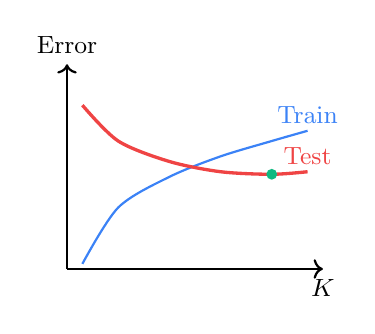
\begin{tikzpicture}[scale=0.65]
  \draw[->, thick] (0,0) -- (5,0) node[below] {\small $K$};
  \draw[->, thick] (0,0) -- (0,4) node[above] {\small Error};
  % Train
  \draw[accent, thick, smooth] plot coordinates {(0.3,0.1)(1,1.2)(2,1.8)(3,2.2)(4,2.5)(4.7,2.7)};
  \node[accent] at (4.7, 3.0) {\small Train};
  % Test
  \draw[softred, very thick, smooth] plot coordinates {(0.3,3.2)(1,2.5)(2,2.1)(3,1.9)(4,1.85)(4.7,1.9)};
  \node[softred] at (4.7, 2.2) {\small Test};
  \fill[softgreen] (4, 1.85) circle (3pt);
\end{tikzpicture}

\vspace{0.3em}
\footnotesize Note: $1/K$ is the flexibility\\
(small $K$ = more flexible)
\end{columns}
\end{frame}


\begin{frame}{Logistic Regression: Assumptions}
\begin{columns}
\column{0.55\textwidth}
\textbf{What logistic regression assumes:}

\begin{enumerate}
  \item Log-odds is \textbf{linear} in $X$
  \item Observations are \textbf{independent}
  \item No \textbf{perfect multicollinearity}
  \item Sample size is \textbf{adequate}\\
    (rule of thumb: $\geq 10$ events per predictor)
\end{enumerate}

\vspace{0.3em}
\textbf{What it does NOT assume:}
\begin{itemize}
  \item Normal distribution of $X$
  \item Constant variance
  \item Linear relationship between $X$ and $Y$
\end{itemize}

\column{0.4\textwidth}
\textbf{Checking assumptions:}

\begin{itemize}
  \item Linearity of logit: plot log-odds vs.\ $X$
  \item VIF for collinearity
  \item Deviance residuals
  \item Hosmer-Lemeshow test
\end{itemize}

\vspace{0.5em}
\textit{Logistic is more flexible than\\LDA --- fewer distributional\\assumptions}
\end{columns}
\end{frame}


\begin{frame}{Deviance: The Logistic Version of RSS}

\textbf{In linear regression:} quality = RSS

\textbf{In logistic regression:} quality = \textbf{Deviance}

$$D = -2 \sum_{i=1}^n \left[y_i \log(\hat{p}_i) + (1-y_i)\log(1-\hat{p}_i)\right]$$

\begin{columns}
\column{0.5\textwidth}
\begin{itemize}
  \item Lower deviance = better fit
  \item Analogous to RSS
  \item Can compare nested models:\\
    $\Delta D \sim \chi^2_{\Delta p}$
  \item Null deviance: model with intercept only
  \item Residual deviance: our model
\end{itemize}

\column{0.45\textwidth}
\textbf{R output:}

\vspace{0.3em}
\footnotesize\texttt{Null deviance: 2920.6}

\texttt{Residual deviance: 1596.5}

\texttt{AIC: 1600.5}
\normalsize

\vspace{0.3em}
Deviance dropped by $1324$\\
$\Rightarrow$ balance is very informative!
\end{columns}
\end{frame}


\begin{frame}{Multinomial Logistic vs.\ LDA for $K > 2$}

\begin{columns}
\column{0.48\textwidth}
\textbf{Multinomial logistic:}
\begin{itemize}
  \item Directly models $P(Y = k \mid X)$
  \item No distributional assumptions
  \item Softmax function
  \item More robust
\end{itemize}

\vspace{0.3em}
R: \texttt{nnet::multinom(y \textasciitilde{} x)}

\column{0.48\textwidth}
\textbf{LDA ($K > 2$):}
\begin{itemize}
  \item Assumes Gaussian within each class
  \item Estimates $K$ means + shared $\boldsymbol{\Sigma}$
  \item More efficient if assumptions hold
  \item Provides nice visualizations
\end{itemize}

\vspace{0.3em}
R: \texttt{MASS::lda(y \textasciitilde{} x)}
\end{columns}

\vspace{0.5em}
\centering
\textit{For $K = 2$: Use \texttt{glm(family=binomial)} --- simpler and standard}
\end{frame}


\begin{frame}{The Role of Priors: A Bayesian Perspective}

\begin{columns}
\column{0.55\textwidth}
$$P(Y = k \mid X) = \frac{\textcolor{accent}{\pi_k} \cdot f_k(x)}{\sum_l \pi_l \cdot f_l(x)}$$

$\pi_k$ = \textcolor{accent}{\textbf{prior}} probability

\vspace{0.3em}
\textbf{Default: use sample proportions}

$\hat{\pi}_k = n_k / n$

\vspace{0.3em}
\textbf{But you can adjust!}

\begin{itemize}
  \item Know disease prevalence? Set $\pi_k$ accordingly
  \item Want to be conservative? Increase prior for ``dangerous'' class
\end{itemize}

\column{0.4\textwidth}
\textbf{Example:}

Default rate $= 3.3\%$

\vspace{0.3em}
With $\hat{\pi}_{\text{Yes}} = 0.033$:

Boundary at balance $\approx \$1{,}800$

\vspace{0.3em}
With $\pi_{\text{Yes}} = 0.5$ (equal priors):

Boundary at balance $\approx \$1{,}200$

\vspace{0.3em}
\textcolor{softgreen}{More conservative: catches more defaulters at cost of more false positives}
\end{columns}
\end{frame}


\begin{frame}{Cross-Validation Preview: How to Choose the Best Method}

\begin{columns}
\column{0.55\textwidth}
\textbf{Problem:}

We compared 5 methods on Smarket\\
but used a \textbf{single} train/test split

\vspace{0.3em}
Results depend on which split!

\vspace{0.5em}
\textbf{Solution (Week 3):}

\textbf{$k$-fold cross-validation}

\begin{enumerate}
  \item Split data into $k$ folds
  \item Train on $k-1$, test on 1
  \item Repeat $k$ times
  \item Average test errors
\end{enumerate}

\column{0.4\textwidth}
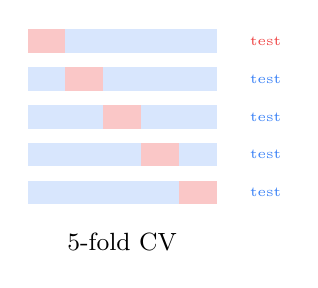
\begin{tikzpicture}[scale=0.6]
  % 5 folds
  \foreach \i in {0,...,4} {
    \fill[accent!20] (0, {3.5-\i*0.8}) rectangle (4, {4-\i*0.8});
    \fill[softred!30] ({\i*0.8}, {3.5-\i*0.8}) rectangle ({(\i+1)*0.8}, {4-\i*0.8});
  }
  \node at (2, -0.5) {\small 5-fold CV};
  \node[softred, right] at (4.5, 3.75) {\tiny test};
  \node[accent, right] at (4.5, 2.95) {\tiny test};
  \node[accent, right] at (4.5, 2.15) {\tiny test};
  \node[accent, right] at (4.5, 1.35) {\tiny test};
  \node[accent, right] at (4.5, 0.55) {\tiny test};
\end{tikzpicture}

\vspace{0.3em}
More reliable estimate of test error!
\end{columns}
\end{frame}


\begin{frame}{Quick Quiz: Test Yourself!}
\begin{enumerate}
  \item What is $P(\text{default})$ if the log-odds is $-3$?
  \pause
  \item[]{\textcolor{muted}{\footnotesize $p = e^{-3}/(1+e^{-3}) = 0.0474 \approx 4.7\%$}}

  \vspace{0.3em}
  \item LDA assumes common $\boldsymbol{\Sigma}$. QDA does not. Which has more parameters?
  \pause
  \item[]{\textcolor{muted}{\footnotesize QDA --- estimates $K$ separate covariance matrices}}

  \vspace{0.3em}
  \item Sensitivity = 90\%, Specificity = 60\%. What happens if we raise the threshold?
  \pause
  \item[]{\textcolor{muted}{\footnotesize Sensitivity decreases, Specificity increases}}

  \vspace{0.3em}
  \item A classifier always predicts ``No'' on imbalanced data. Accuracy = 97\%. Good?
  \pause
  \item[]{\textcolor{muted}{\footnotesize No --- sensitivity = 0\%, it misses all positives. Check AUC or F1.}}
\end{enumerate}
\end{frame}


\begin{frame}{Quick Quiz: More Questions}
\begin{enumerate}
  \setcounter{enumi}{4}
  \item When would you prefer LDA over logistic regression?
  \pause
  \item[]{\textcolor{muted}{\footnotesize When classes are well-separated Gaussians, especially with small $n$}}

  \vspace{0.3em}
  \item Why is Naive Bayes ``naive''?
  \pause
  \item[]{\textcolor{muted}{\footnotesize It assumes all predictors are independent given the class --- rarely true}}

  \vspace{0.3em}
  \item You fit KNN with $K=1$. Training error?
  \pause
  \item[]{\textcolor{muted}{\footnotesize Exactly 0\% --- each point is its own nearest neighbor}}

  \vspace{0.3em}
  \item ROC curve hugs the top-left corner. Is this good or bad?
  \pause
  \item[]{\textcolor{muted}{\footnotesize Good --- high TPR with low FPR at many thresholds. AUC $\approx 1$}}
\end{enumerate}
\end{frame}


\begin{frame}{Common Mistakes in Classification}

\begin{enumerate}
  \item \textbf{Using accuracy on imbalanced data}
  \begin{itemize}
    \item[$\circ$] Always report sensitivity, specificity, AUC
  \end{itemize}

  \vspace{0.3em}
  \item \textbf{Evaluating on training data}
  \begin{itemize}
    \item[$\circ$] Always use a held-out test set or CV
  \end{itemize}

  \vspace{0.3em}
  \item \textbf{Ignoring the threshold}
  \begin{itemize}
    \item[$\circ$] 0.5 is default, not optimal. Tune it!
  \end{itemize}

  \vspace{0.3em}
  \item \textbf{Coding $K > 2$ classes as numbers for linear regression}
  \begin{itemize}
    \item[$\circ$] Use logistic / LDA / softmax instead
  \end{itemize}

  \vspace{0.3em}
  \item \textbf{Forgetting to standardize for KNN}
  \begin{itemize}
    \item[$\circ$] KNN uses distances --- scale matters!
  \end{itemize}
\end{enumerate}
\end{frame}


\begin{frame}{GLM Family: The Bigger Picture}

\begin{center}
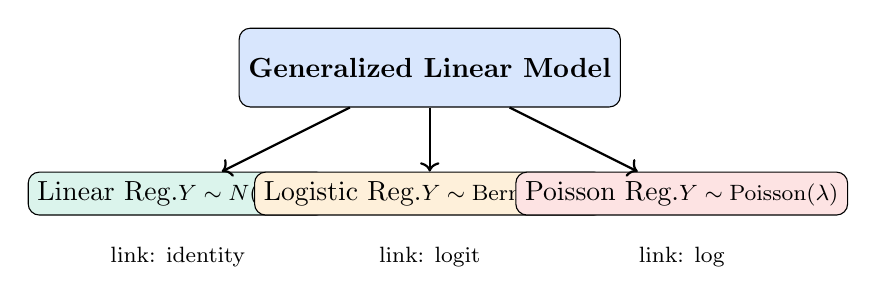
\begin{tikzpicture}[scale=0.8]
  \node[draw, fill=accent!20, rounded corners, minimum width=4cm, minimum height=1cm, font=\bfseries] (glm) at (0,3) {Generalized Linear Model};
  \node[draw, fill=softgreen!15, rounded corners, minimum width=3cm] (lr) at (-4,1) {Linear Reg.\\ \footnotesize $Y \sim N(\mu, \sigma^2)$};
  \node[draw, fill=amber!15, rounded corners, minimum width=3cm] (log) at (0,1) {Logistic Reg.\\ \footnotesize $Y \sim \text{Bernoulli}(p)$};
  \node[draw, fill=softred!15, rounded corners, minimum width=3cm] (poi) at (4,1) {Poisson Reg.\\ \footnotesize $Y \sim \text{Poisson}(\lambda)$};
  \draw[->, thick] (glm) -- (lr);
  \draw[->, thick] (glm) -- (log);
  \draw[->, thick] (glm) -- (poi);
  \node[below, font=\footnotesize] at (-4, 0.3) {link: identity};
  \node[below, font=\footnotesize] at (0, 0.3) {link: logit};
  \node[below, font=\footnotesize] at (4, 0.3) {link: log};
\end{tikzpicture}
\end{center}

\vspace{0.3em}
All three: $g(E[Y]) = \beta_0 + \beta_1 X_1 + \cdots + \beta_p X_p$

R: \texttt{glm(y \textasciitilde{} x, family = gaussian / binomial / poisson)}
\end{frame}


\begin{frame}{Summary: Chapter 4 Key Takeaways}

\begin{columns}
\column{0.48\textwidth}
\begin{itemize}
  \item Don't use linear regression for classification
  \item Logistic regression: model $P(Y \mid X)$ via sigmoid
  \item Coefficients: change in \textbf{log-odds} per unit $X$
  \item MLE estimation (not least squares)
\end{itemize}

\column{0.48\textwidth}
\begin{itemize}
  \item LDA: Gaussian classes, shared $\boldsymbol{\Sigma}$
  \item QDA: Gaussian classes, separate $\boldsymbol{\Sigma}_k$
  \item Naive Bayes: independence assumption
  \item KNN: non-parametric, curse of dimensionality
  \item ROC + AUC for evaluation
\end{itemize}
\end{columns}

\vspace{0.8em}
\centering
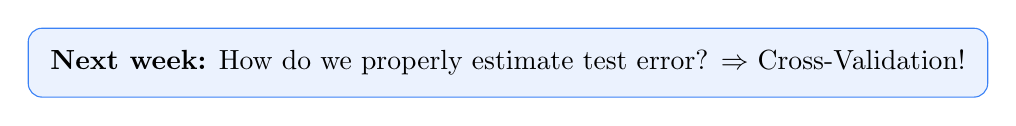
\begin{tikzpicture}
\node[fill=accent!10, rounded corners=5pt, inner sep=8pt, draw=accent] {
  \textbf{Next week:} How do we properly estimate test error? $\Rightarrow$ Cross-Validation!
};
\end{tikzpicture}
\end{frame}


% ═══════════ EXERCISES ═══════════
\begin{frame}{Exercise 1: Default Data (ISLR 4.8 Q13)}

\textbf{Data:} \texttt{Default} \hfill $n = 10{,}000$

\begin{enumerate}
  \item Fit logistic regression: \texttt{default \textasciitilde{} income + balance}
  \item Split into train/test (use \texttt{set.seed(1)})
  \item Compute test error rate
  \item Repeat with different random splits --- does error vary?
  \item Add \texttt{student} as a predictor --- does it improve?
\end{enumerate}

\vspace{0.3em}
\fbox{\textbf{Hint:} Test error should be around 2.5--3.5\%}
\end{frame}


\begin{frame}{Exercise 2: Smarket Data (ISLR 4.8 Q10)}

\textbf{Data:} \texttt{Smarket} \hfill Predict: \texttt{Direction}

\begin{enumerate}
  \item EDA: Produce numerical and graphical summaries
  \item Fit logistic regression using all Lag variables + Volume
  \item Confusion matrix and accuracy on training data
  \item Fit using only Lag1 + Lag2 (train: 2001--2004, test: 2005)
  \item Repeat with LDA, QDA, KNN ($K = 1, 3, 5$)
  \item Which method gives the best test accuracy?
\end{enumerate}

\vspace{0.3em}
\fbox{\textbf{Key finding:} QDA achieves $\approx 60\%$ accuracy}
\end{frame}


\begin{frame}{Exercise 3: Weekly Data (ISLR 4.8 Q11)}

\textbf{Data:} \texttt{Weekly} \hfill $n = 1{,}089$ weekly returns

\begin{enumerate}
  \item EDA: patterns in Lag1--Lag5 and Volume?
  \item Fit logistic regression with all Lag variables + Volume
  \item Confusion matrix --- what is the overall error rate?
  \item Fit using only Lag2 (train: 1990--2008, test: 2009--2010)
  \item Repeat with LDA, QDA, KNN ($K = 5$)
  \item Compare results --- which performs best?
\end{enumerate}
\end{frame}


\begin{frame}{Exercise 4: Boston Crime (ISLR 4.8 Q16)}

\textbf{Data:} \texttt{Boston} \hfill Create binary: \texttt{crim > median}

\begin{enumerate}
  \item Create binary response: \texttt{high\_crime <- ifelse(crim > median(crim), 1, 0)}
  \item Explore predictors with boxplots and correlations
  \item Fit logistic regression, LDA, KNN (try various $K$)
  \item Which predictors are most useful?
  \item Which method gives the best test accuracy?
\end{enumerate}

\vspace{0.3em}
\fbox{\textbf{Hint:} \texttt{rad}, \texttt{tax}, \texttt{nox}, \texttt{lstat} should be strong predictors}
\end{frame}


% ═══════════ SOLUTIONS ═══════════
\begin{frame}{Solution: Exercise 1 --- Default}
\begin{columns}
\column{0.5\textwidth}
\texttt{balance}: $\hat{\beta} = 0.0057$, $p < 0.001$

\texttt{income}: $\hat{\beta} = 0.003$, $p = 0.62$

\textcolor{softred}{Income is not significant!}

\vspace{0.3em}
Test error $\approx 2.7\%$ (varies by split)

\vspace{0.3em}
Adding \texttt{student} reduces error slightly\\
but effect is small

\column{0.45\textwidth}
\textbf{Confusion matrix (typical):}

\vspace{0.3em}
\begin{tabular}{lcc}
\toprule
 & Pred.\ No & Pred.\ Yes \\
\midrule
No & 2,413 & 12 \\
Yes & 60 & 15 \\
\bottomrule
\end{tabular}

\vspace{0.3em}
Sensitivity $\approx 20\%$

\footnotesize Low, because defaults are rare
\end{columns}
\end{frame}


\begin{frame}{Solution: Exercise 2 --- Smarket}
\begin{columns}
\column{0.55\textwidth}
\textbf{Key results (test 2005):}

\begin{tabular}{lc}
\toprule
Method & Accuracy \\
\midrule
Logistic (Lag1, Lag2) & 56.1\% \\
LDA (Lag1, Lag2) & 56.0\% \\
\textcolor{softgreen}{QDA (Lag1, Lag2)} & \textcolor{softgreen}{59.9\%} \\
KNN $K=1$ & 50.0\% \\
KNN $K=3$ & 53.6\% \\
\bottomrule
\end{tabular}

\column{0.4\textwidth}
\textbf{Insights:}

\begin{itemize}
  \item Using all Lags: no predictor is significant
  \item Lag1 + Lag2 only: slight improvement
  \item QDA best: suggests non-linear boundary
  \item KNN $K=1$ = pure noise
\end{itemize}
\end{columns}
\end{frame}


\begin{frame}{Solution: Exercise 3 --- Weekly}
\begin{columns}
\column{0.5\textwidth}
\textbf{EDA findings:}
\begin{itemize}
  \item Volume increases over time
  \item Lag variables: no clear pattern
  \item Only Lag2 is marginally significant
\end{itemize}

\vspace{0.3em}
\textbf{Best model:}

Logistic with Lag2 only: $62.5\%$ accuracy

LDA: $62.5\%$ (identical)

\column{0.45\textwidth}
\textbf{Confusion matrix (Logistic):}

\vspace{0.3em}
\begin{tabular}{lcc}
\toprule
 & Pred.\ Down & Pred.\ Up \\
\midrule
Down & 9 & 34 \\
Up & 5 & 56 \\
\bottomrule
\end{tabular}

\vspace{0.3em}
Model mostly predicts ``Up''

Good at catching Up days\\
but poor at Down days
\end{columns}
\end{frame}


\begin{frame}{Solution: Exercise 4 --- Boston Crime}
\begin{columns}
\column{0.5\textwidth}
\textbf{Strong predictors:}

\texttt{nox}, \texttt{rad}, \texttt{tax}, \texttt{dis}, \texttt{lstat}, \texttt{age}

\vspace{0.3em}
\textbf{Best methods:}

\begin{tabular}{lc}
\toprule
Method & Accuracy \\
\midrule
Logistic & $\sim 87\%$ \\
LDA & $\sim 86\%$ \\
KNN $K=3$ & $\sim 89\%$ \\
KNN $K=10$ & $\sim 87\%$ \\
\bottomrule
\end{tabular}

\column{0.45\textwidth}
\textbf{Insights:}

\begin{itemize}
  \item KNN with small $K$ performs best
  \item Suggests non-linear boundaries
  \item \texttt{nox} and \texttt{rad} are the strongest single predictors
  \item Crime is well-predicted by socioeconomic variables
\end{itemize}
\end{columns}
\end{frame}


% ═══════════ CLOSING ═══════════
\begin{frame}{What's Next?}

\begin{center}
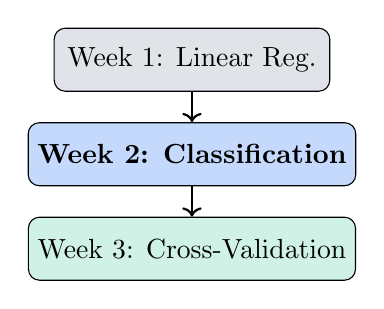
\begin{tikzpicture}[scale=0.8]
  \node[draw, fill=muted!20, rounded corners, minimum width=3.5cm, minimum height=0.8cm] (w1) at (0,0) {Week 1: Linear Reg.};
  \node[draw, fill=accent!30, rounded corners, minimum width=3.5cm, minimum height=0.8cm, font=\bfseries] (w2) at (0,-1.5) {Week 2: Classification};
  \node[draw, fill=softgreen!20, rounded corners, minimum width=3.5cm, minimum height=0.8cm] (w3) at (0,-3.0) {Week 3: Cross-Validation};
  \draw[->, thick] (w1) -- (w2);
  \draw[->, thick] (w2) -- (w3);
\end{tikzpicture}
\end{center}

\vspace{0.3em}
\textbf{Homework:} ISLR Chapter 4: Q10, 11, 13, 16

\textbf{Lab:} \texttt{Lab\_Week02.R} --- Logistic, LDA, QDA, NB, KNN on Default + Smarket

\textbf{Next week:} How do we \textit{properly} estimate test error? $\Rightarrow$ Cross-Validation!
\end{frame}


\begin{frame}{}
\centering
\vspace{2cm}
{\Huge\textbf{Thank You}}

\vspace{1em}
{\Large Questions?}

\vspace{1.5em}
{\large Dr.\ Endri Ra\c{c}o \quad|\quad Machine Learning with R}

\vspace{0.5em}
{\normalsize \texttt{github.com/endri81/ISLRv2-solutions}}
\end{frame}

\end{document}
